%==============================================================================
%  SCE 672 Advanced Robotics (Term 261) - Project Phase 3 Technical Report
%  RoboMaster Odometry: EKF prediction with wheel odometry, correction with an AprilTag
%  Overleaf: upload overleaf_upload.zip (main.tex, sections/, figures/, kfupm_logo.png),
%  compile with pdfLaTeX. Figures and tables come from scripts/analyze_trials.py and scripts/replay_ekf.py.
%==============================================================================
\documentclass[11pt,a4paper]{article}

%------------------------------ STUDENT DETAILS -------------------------------
\newcommand{\studentName}{Ziad Aboelkhir}
\newcommand{\studentID}{g202622300}
\newcommand{\studentProgram}{Ph.D. (Direct), Systems \& Control Engineering}
\newcommand{\studentDept}{Control \& Instrumentation Engineering (CIE)}
\newcommand{\instructor}{Prof.\ Aamer Iqbal Bhatti}
\newcommand{\courseCode}{SCE 672}
\newcommand{\courseName}{Advanced Robotics}
\newcommand{\termLine}{Term 261 (Fall 2026)}
\newcommand{\submitDate}{November 15, 2026}
\newcommand{\repoURL}{https://github.com/Ziad-Behairy/SCE672-Phase3-RoboMaster-Odometry}
% >>> PLACEHOLDER: replace with the YouTube link of results/video/phase3_demo.mp4 <<<
\newcommand{\videolink}{VIDEO-LINK-TBD}

%-------------------------------- PACKAGES ------------------------------------
\usepackage[a4paper,top=2.3cm,bottom=2.3cm,left=2.2cm,right=2.2cm,headheight=16pt]{geometry}
\usepackage[T1]{fontenc}
\usepackage{lmodern}
\usepackage{microtype}
\DisableLigatures[-]{encoding = T1, family = tt*}
\linespread{1.04}
\usepackage{graphicx}
\usepackage[table]{xcolor}
\usepackage{fontawesome5}
\usepackage{tabularx,booktabs,array,multirow}
\usepackage{enumitem}
\usepackage[most]{tcolorbox}
\usepackage{amsmath,amssymb,bm}
\usepackage{tikz}
\usetikzlibrary{arrows.meta,positioning,calc,fit,backgrounds,shapes.geometric,shapes.misc,decorations.pathreplacing,patterns}
\usepackage{listings}
\usepackage{caption}
\usepackage{subcaption}
\usepackage{float}
\usepackage{titlesec}
\usepackage{fancyhdr}
\usepackage[hidelinks]{hyperref}

%--------------------------------- COLOURS ------------------------------------
\definecolor{kfupm}{RGB}{12,126,64}
\definecolor{kfupmdark}{RGB}{6,84,42}
\definecolor{kfupmlight}{RGB}{233,244,237}
\definecolor{ink}{RGB}{33,37,41}
\definecolor{muted}{RGB}{105,112,120}
\definecolor{warn}{RGB}{176,96,0}
\definecolor{alert}{RGB}{190,50,45}
\definecolor{accblue}{HTML}{2A78D6}
\definecolor{accorange}{HTML}{EB6834}
\definecolor{accpurple}{HTML}{7B3FA0}
\definecolor{accgold}{HTML}{D4A017}
\definecolor{accgreen}{HTML}{0B7A3E}
\definecolor{accred}{HTML}{C0392B}
\definecolor{codebg}{RGB}{246,248,247}
% controller states (same colors as the video)
\definecolor{cWAITING}{HTML}{D4A017}
\definecolor{cDRIVING}{HTML}{2A78D6}
\definecolor{cHOLDING}{HTML}{7B3FA0}
\definecolor{cDONE}{HTML}{0B7A3E}
\color{ink}

\hypersetup{
  colorlinks=true, linkcolor=kfupm, urlcolor=kfupm, citecolor=kfupm,
  pdftitle={SCE 672 Project Phase 3: RoboMaster odometry with an Extended Kalman Filter},
  pdfauthor={\studentName}, pdfsubject={SCE 672 Advanced Robotics, Project Phase 3},
  pdfkeywords={RoboMaster EP, ROS 2 Jazzy, AprilTag, odometry, Extended Kalman Filter, prediction, correction}
}

%---------------------------------- LAYOUT ------------------------------------
\setlength{\parindent}{0pt}
\setlength{\parskip}{5pt}
\raggedbottom
\setlength{\intextsep}{9pt plus 2pt minus 2pt}
\setlist{itemsep=2pt,parsep=0pt,topsep=3pt,leftmargin=1.4em,labelsep=0.5em}
\setlist[itemize]{label=\textcolor{kfupm}{\scriptsize\faCaretRight}}
\setlist[enumerate]{label=\textcolor{kfupm}{\bfseries\arabic*.}}
\renewcommand{\arraystretch}{1.25}
\DeclareRobustCommand{\code}[1]{\texttt{\detokenize{#1}}}
\newcommand{\link}[2]{\href{#1}{\textcolor{kfupm}{#2}}}
\newcommand{\hd}[1]{\textcolor{white}{\bfseries #1}}      % table header cell
\newcommand{\lead}[1]{\textbf{\color{kfupmdark}#1}\enspace}  % run-in paragraph lead
\newcommand{\stbadge}[1]{{\setlength{\fboxsep}{1.6pt}\colorbox{c#1!16}{\textcolor{c#1}{\scriptsize\bfseries\sffamily #1}}}}
\newcommand{\dest}{\hat d}

% section style: green numbered badge + title + thin rule
\titleformat{\section}[hang]{\normalfont\LARGE\bfseries\color{kfupmdark}}
  {\tikz[baseline=(b.base)]\node[fill=kfupm,text=white,rounded corners=3pt,inner sep=4pt,
     minimum width=20pt,font=\Large\bfseries](b){\thesection};}{10pt}{}
  [\vspace{2pt}{\color{kfupm!45}\titlerule[0.8pt]}]
\titleformat{\subsection}{\normalfont\Large\bfseries\color{kfupm}}{\thesubsection}{9pt}{}
\titlespacing*{\section}{0pt}{14pt}{8pt}
\titlespacing*{\subsection}{0pt}{10pt}{4pt}
\newcommand{\isec}[2]{\section{\texorpdfstring{\textcolor{kfupm}{#1}\hspace{8pt}}{}#2}}
\newcommand{\isub}[2]{\subsection{\texorpdfstring{\textcolor{kfupm}{\normalsize #1}\hspace{6pt}}{}#2}}

% header and footer
\pagestyle{fancy}
\fancyhf{}
\renewcommand{\headrulewidth}{0.6pt}
\renewcommand{\headrule}{\hbox to\headwidth{\color{kfupm!50}\leaders\hrule height \headrulewidth\hfill}}
\fancyhead[L]{\small\color{kfupmdark}\faRobot\ \courseCode\ \courseName\ \textbullet\ Project Phase 3}
\fancyhead[R]{\small\color{muted}\studentName\ \textbullet\ \studentID}
\fancyfoot[C]{\small\color{kfupm}\bfseries\thepage}
\fancyfoot[R]{\scriptsize\color{muted}KFUPM \textbullet\ CIE}

% captions
\captionsetup{font=small,labelfont={bf,color=kfupmdark},labelsep=period,skip=5pt}
\captionsetup[sub]{font=footnotesize}

% boxes
\newtcolorbox{keybox}[2][]{enhanced,colback=kfupmlight,colframe=kfupm,arc=2.5pt,boxrule=0.7pt,
  left=7pt,right=7pt,top=4pt,bottom=5pt,fonttitle=\bfseries\small,coltitle=white,
  title={#2},attach boxed title to top left={xshift=7pt,yshift=-2mm},
  boxed title style={colback=kfupm,arc=2pt,boxrule=0pt},before skip=10pt,after skip=8pt,#1}
\newtcolorbox{bluebox}[2][]{enhanced,colback=accblue!5,colframe=accblue!80,arc=2.5pt,boxrule=0.7pt,
  left=7pt,right=7pt,top=4pt,bottom=5pt,fonttitle=\bfseries\small,coltitle=white,
  title={#2},attach boxed title to top left={xshift=7pt,yshift=-2mm},
  boxed title style={colback=accblue,arc=2pt,boxrule=0pt},before skip=10pt,after skip=8pt,#1}
\newtcolorbox{purplebox}[2][]{enhanced,colback=accpurple!5,colframe=accpurple!80,arc=2.5pt,boxrule=0.7pt,
  left=7pt,right=7pt,top=4pt,bottom=5pt,fonttitle=\bfseries\small,coltitle=white,
  title={#2},attach boxed title to top left={xshift=7pt,yshift=-2mm},
  boxed title style={colback=accpurple,arc=2pt,boxrule=0pt},before skip=10pt,after skip=8pt,#1}
\newtcolorbox{notebox}[1][]{enhanced,colback=white,colframe=kfupm!55,arc=2pt,boxrule=0.5pt,
  borderline west={2.6pt}{0pt}{kfupm},left=8pt,right=7pt,top=4pt,bottom=4pt,
  before skip=8pt,after skip=8pt,#1}
\newtcolorbox{warnbox}[1][]{enhanced,colback=warn!6,colframe=warn!70,arc=2pt,boxrule=0.5pt,
  borderline west={2.6pt}{0pt}{warn},left=8pt,right=7pt,top=4pt,bottom=4pt,
  before skip=8pt,after skip=8pt,#1}
\newcommand{\stat}[4][kfupm]{%
  \begin{tcolorbox}[enhanced,width=0.235\linewidth,nobeforeafter,colback=white,colframe=#1!60,
    borderline north={2.5pt}{0pt}{#1},arc=3pt,boxrule=0.6pt,halign=center,valign=center,height=2.4cm,left=2pt,right=2pt]
  {\color{#1}\Large #2}\\[3pt]{\color{kfupmdark}\Large\bfseries #3}\\[2pt]{\footnotesize\color{muted}#4}
  \end{tcolorbox}}

% code listings
\lstdefinestyle{sh}{language=bash,basicstyle=\ttfamily\footnotesize,backgroundcolor=\color{codebg},
  frame=leftline,framerule=2.6pt,rulecolor=\color{kfupm},xleftmargin=9pt,framexleftmargin=7pt,
  keywordstyle=\color{kfupmdark}\bfseries,commentstyle=\color{muted}\itshape,stringstyle=\color{warn},
  showstringspaces=false,columns=fullflexible,keepspaces=true,breaklines=true,upquote=true,
  aboveskip=8pt,belowskip=6pt}
\lstdefinestyle{py}{language=Python,basicstyle=\ttfamily\footnotesize,backgroundcolor=\color{codebg},
  frame=leftline,framerule=2.6pt,rulecolor=\color{accblue},xleftmargin=9pt,framexleftmargin=7pt,
  keywordstyle=\color{accblue}\bfseries,commentstyle=\color{muted}\itshape,stringstyle=\color{warn},
  showstringspaces=false,columns=fullflexible,keepspaces=true,breaklines=true,upquote=true,
  numbers=left,numberstyle=\tiny\color{muted},numbersep=6pt,aboveskip=8pt,belowskip=6pt}

% tikz styles
\tikzset{
  blk/.style={draw=kfupm,fill=kfupmlight,rounded corners=3pt,align=center,inner sep=5pt,
              font=\small,text width=#1},
  blk/.default=4cm,
  grp/.style={draw=kfupmdark,thick,rounded corners=6pt,inner sep=9pt},
  arr/.style={-{Latex[length=2.4mm]},thick,color=kfupmdark},
  topic/.style={draw=muted,fill=white,rounded corners=1pt,font=\footnotesize\ttfamily,inner sep=3pt},
  rosnode/.style={draw=kfupm,fill=kfupmlight,rounded corners=3pt,font=\footnotesize\ttfamily,inner sep=4pt},
  lbl/.style={font=\scriptsize,color=muted,align=center},
  stnode/.style={draw=c#1,fill=c#1!10,line width=1.1pt,rounded corners=6pt,align=center,
                 inner sep=5pt,text width=3.3cm,font=\small},
  tr/.style={-{Latex[length=2.6mm]},thick,color=ink},
  trl/.style={font=\scriptsize,align=center,fill=white,inner sep=1.5pt}
}

%==============================================================================
\begin{document}

%================================= COVER ======================================
\begin{titlepage}
\newgeometry{top=0cm,bottom=0cm,left=0cm,right=0cm}
\thispagestyle{empty}
\begin{tikzpicture}[remember picture,overlay]
  \fill[kfupm] (current page.north west) rectangle ([yshift=-6.3cm]current page.north east);
  \fill[kfupmdark] ([yshift=-6.3cm]current page.north west) rectangle ([yshift=-6.55cm]current page.north east);
  % thin colored strip with the four controller states
  \foreach \col [count=\i from 0] in {cWAITING,cDRIVING,cHOLDING,cDONE}{
    \fill[fill=\col] ([xshift=\i*5.25cm,yshift=-6.55cm]current page.north west) rectangle
              ([xshift=\i*5.25cm+5.25cm,yshift=-6.75cm]current page.north west);}
  \fill[kfupm] (current page.south west) rectangle ([yshift=1.3cm]current page.south east);
  \node[fill=white,circle,inner sep=10pt,draw=kfupmdark,line width=2pt] at ([yshift=-6.4cm]current page.north)
       {
\includegraphics[width=3.9cm]{kfupm_logo.png}};
  \node[text=white,align=center,font=\Large\bfseries] at ([yshift=-1.55cm]current page.north)
       {King Fahd University of Petroleum \& Minerals};
  \node[text=white,align=center,font=\large] at ([yshift=-2.35cm]current page.north)
       {College of Engineering and Physics \textbullet\ \studentDept};
  \node[text=white,align=center,font=\normalsize] at ([yshift=0.65cm]current page.south)
       {\faUniversity\ Dhahran, Saudi Arabia \quad\textbullet\quad \submitDate};
\end{tikzpicture}
\vspace*{10.2cm}
\begin{center}
  {\color{kfupm}\large\bfseries \courseCode\ \textbullet\ \courseName\ \textbullet\ \termLine\par}
  \vspace{0.45cm}
  {\color{kfupmdark}\fontsize{26}{31}\selectfont\bfseries Project Phase 3 Technical Report\par}
  \vspace{0.35cm}
  {\Large RoboMaster Odometry:\\[3pt] Prediction and Correction with an Extended Kalman Filter\par}
  \vspace{0.3cm}
  {\color{muted}\large Drive straight to a floor AprilTag, stop at 0.50\,m and estimate the distance throughout,\\
   on the DJI RoboMaster EP Core with ROS 2 Jazzy\par}
  \vspace{0.8cm}
  \begin{minipage}{16.4cm}
  \stat[kfupm]{\faBullseye}{0.28\,cm}{MAE of the final distance}\hfill
  \stat[accblue]{\faRulerHorizontal}{0.96\,cm}{range of errors}\hfill
  \stat[accgreen]{\faCheckDouble}{10 / 10}{valid trials, same start}\hfill
  \stat[accorange]{\faCogs}{1.98\,cm}{MAE with wheels alone}
  \end{minipage}
  \vspace{0.8cm}

  \begin{tcolorbox}[center,width=14.2cm,colback=kfupmlight,colframe=kfupm,arc=3pt,boxrule=0.8pt,left=10pt,right=10pt]
  \large
  \begin{tabular}{@{}c@{\hspace{9pt}}l@{\hspace{12pt}}l@{}}
   \textcolor{kfupm}{\faUserGraduate}      & Student     & \textbf{\studentName}\\
   \textcolor{kfupm}{\faIdCard}            & Student ID  & \studentID\\
   \textcolor{kfupm}{\faGraduationCap}     & Program     & \studentProgram\\
   \textcolor{kfupm}{\faChalkboardTeacher} & Instructor  & \instructor\\
   \textcolor{kfupm}{\faRobot}             & Platform    & RoboMaster EP Core, ROS 2 Jazzy, Ubuntu 24.04\\
   \textcolor{kfupm}{\faCalendarCheck}     & Submitted   & \submitDate
  \end{tabular}
  \end{tcolorbox}
\end{center}
\restoregeometry
\end{titlepage}

%============================ CONTENTS & MAP =================================
\setcounter{page}{2}
{\hypersetup{linkcolor=ink}\setcounter{tocdepth}{2}\tableofcontents}
\clearpage

\begin{keybox}{\faClipboardCheck\ \ Required work and where it is answered}
\small
\begin{tabularx}{\linewidth}{@{}>{\raggedright\arraybackslash}p{4.6cm}>{\raggedright\arraybackslash}X>{\raggedright\arraybackslash}p{2.6cm}@{}}
\textbf{Spec item} & \textbf{Answer} & \textbf{Location}\\\midrule
1. Tag detection, straight-line motion, prediction, correction; sensors used for correction
  & AprilTag range/bearing from the camera; heading-hold controller; 5-state EKF predicted with a unicycle model,
    corrected by \code{/odom} $(v,\omega)$ and by the tag $(d,\varphi)$ & Sections~\ref{sec:method}, \ref{sec:setup}\\
2. 8 to 10 trials, same start, estimated and measured final distance, same reference point
  & 10 trials from 1.20\,m, stop at 0.50\,m; reference point = middle of the chassis front for both & Section~\ref{sec:results}, Table~\ref{tab:trials}\\
3. Error $e = d_{est}-d_{meas}$, MAE and range & MAE 0.28\,cm, range 0.96\,cm (plus bias, $\sigma$, covariance) & Table~\ref{tab:trials}, Section~\ref{sec:stats}\\
4. Table and discussion: consistency, sources of error, role of prediction and correction
  & trial-to-trial spread, seven evidenced error sources, offline replay with each sensor removed & Section~\ref{sec:discussion}\\
Submission: report, code, video & this PDF; \link{\repoURL}{\faGithub\ repository}; \link{\videolink}{\faVideo\ demo video} & Appendix~\ref{sec:repro}\\
\end{tabularx}
\end{keybox}

\begin{notebox}
\small\textbf{\color{kfupmdark}\faInfoCircle\ How the numbers were produced}
\begin{itemize}
  \item Every 50\,ms tick of every trial is logged in \code{results/trials/trial_NN_*/steps.csv} (state, full $P$, gain $K$,
        raw sensor readings); \code{summary.json} holds the final values and the tape measurement.
  \item Table~\ref{tab:trials}, the statistics and Figures~\ref{fig:scatter}--\ref{fig:stats} are generated by
        \code{scripts/analyze_trials.py}; the sensor-removal study (Table~\ref{tab:replay}) by \code{scripts/replay_ekf.py}.
        Nothing was typed in by hand except the tape readings.
  \item The tape readings were taken by the student after each stop, from the middle of the chassis front to the
        centre of the tag, and entered with \code{scripts/add_measurement.py}.
\end{itemize}
\end{notebox}

%============================ 1. OVERVIEW =====================================
\isec{\faCompass}{Problem and Experiment Design}
\label{sec:overview}

The task is to make the RoboMaster EP Core detect a fixed tag, drive straight towards it and stop before it, while
estimating its position with \emph{odometry-based prediction} and \emph{sensor-based correction}. The quantity that is
graded is the final distance to the tag: the robot's own estimate $d_{est}$ is compared with an independent tape
measurement $d_{meas}$ in every trial, $e = d_{est}-d_{meas}$.

\begin{figure}[H]
\centering
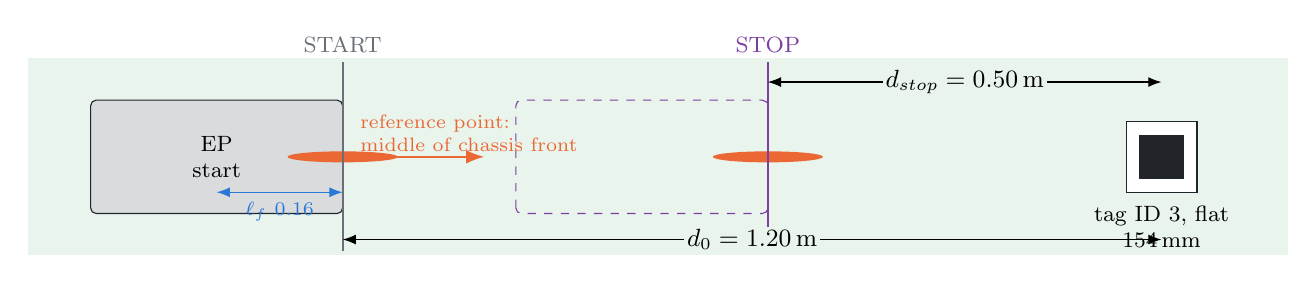
\begin{tikzpicture}[x=10cm,y=1cm,font=\small]
  % floor
  \fill[kfupmlight] (-0.08,-1.25) rectangle (1.52,1.25);
  % tag
  \fill[white,draw=ink] (1.36-0.045,-0.45) rectangle (1.36+0.045,0.45);
  \fill[ink] (1.36-0.028,-0.28) rectangle (1.36+0.028,0.28);
  \node[below,font=\footnotesize] at (1.36,-0.5) {tag ID 3, flat};
  \node[below,font=\footnotesize] at (1.36,-0.85) {154\,mm};
  % robot at start
  \draw[fill=muted!25,draw=ink,rounded corners=2pt] (0,-0.72) rectangle (0.32,0.72);
  \node[font=\footnotesize,align=center] at (0.16,0) {EP\\start};
  \fill[accorange] (0.32,0) circle (0.07);
  % robot at stop (ghost)
  \draw[dashed,draw=accpurple,rounded corners=2pt] (0.54,-0.72) rectangle (0.86,0.72);
  \fill[accorange] (0.86,0) circle (0.07);
  % lines
  \draw[thick,muted] (0.32,-1.2) -- (0.32,1.2) node[above,font=\footnotesize]{START};
  \draw[thick,accpurple] (0.86,-1.2) -- (0.86,1.2) node[above,font=\footnotesize]{STOP};
  % dimensions
  \draw[{Latex}-{Latex}] (0.32,-1.05) -- (1.36,-1.05) node[midway,fill=kfupmlight,inner sep=1pt]{$d_0 = 1.20$\,m};
  \draw[{Latex}-{Latex}] (0.86,0.95) -- (1.36,0.95) node[midway,fill=kfupmlight,inner sep=1pt]{$d_{stop}=0.50$\,m};
  \draw[{Latex}-{Latex},accblue] (0.16,-0.45) -- (0.32,-0.45) node[midway,below,font=\scriptsize]{$\ell_f$ 0.16};
  \draw[-{Latex},thick,accorange] (0.36,0) -- (0.5,0);
  \node[font=\scriptsize,accorange,align=left,anchor=west] at (0.33,0.3) {reference point:\\middle of chassis front};
\end{tikzpicture}
\caption{The experiment, to scale along the path. Every distance in this report is measured from the same reference
point (orange: the middle of the chassis front) to the centre of the tag. The filter tracks the robot centre, which is
$\ell_f = 0.16$\,m behind the reference point; the conversion is done inside the filter (Section~\ref{sec:method}).}
\label{fig:setup}
\end{figure}

\begin{table}[H]
\centering\small
\rowcolors{2}{kfupmlight}{white}
\begin{tabularx}{\linewidth}{@{}l>{\raggedright\arraybackslash}X@{}}
\rowcolor{kfupm}\hd{Choice} & \hd{Value and reason}\\
Start distance $d_0$ & \textbf{1.20\,m} (spec: 1 to 2\,m, recorded and kept for all trials). 1.50\,m was tried first:
  the flat 154\,mm tag is then only about 10 pixels tall in the 720p image and detection came and went (0 of 20
  frames in one check), so the start was moved to 1.20\,m, where the tag is detected in 70 to 75 of 75 frames.\\
Stop distance $d_{stop}$ & \textbf{0.50\,m} (spec: suitable, same for all trials). Below about 0.47\,m the floor tag
  leaves the bottom of the camera image; stopping at 0.50\,m keeps the camera correction active until the end, so the
  final estimate is never pure prediction.\\
Tag & AprilTag tag36h11, ID 3, black square 154\,mm, taped flat on the floor (same print as Phase 2).\\
Reference point & Middle of the chassis front, for both $d_{est}$ and the tape measurement $d_{meas}$.\\
Robot and software & DJI RoboMaster EP Core, Ubuntu 24.04, ROS 2 Jazzy, \code{robomaster_ros} driver in router (STA)
  mode, camera at 720p on the arm at the saved pose $(x,z)=(0.123, 0.067)$\,m.\\
Trials & 10, all from the same taped start marks, same room, floor, light and configuration.\\
\end{tabularx}
\caption{Experiment design.}
\label{tab:design}
\end{table}

\begin{notebox}
\small\lead{Floor.} The trials were run on a woven rug. It is a realistic surface for odometry (the Mecanum rollers
slip a little on it), and it is one of the error sources quantified in Section~\ref{sec:discussion}.
\end{notebox}

%============================ 2. METHOD =======================================
\isec{\faProjectDiagram}{Method: Detection, Prediction, Correction, Control}
\label{sec:method}

\isub{\faSitemap}{System architecture}
Two ROS 2 nodes run next to the DJI driver (Figure~\ref{fig:arch}). \code{tag_detector} turns camera images into a
range and bearing to the tag. \code{phase3_ekf} runs the filter and the controller at 20\,Hz and logs every tick.

\begin{figure}[H]
\centering
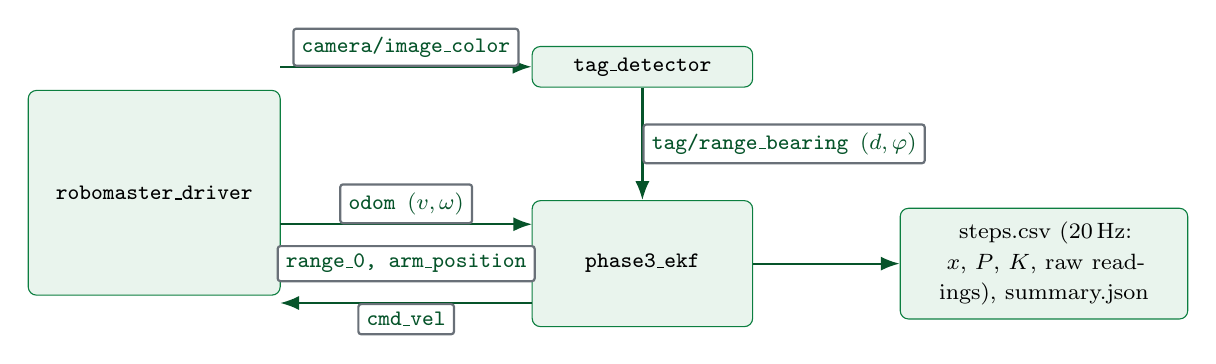
\begin{tikzpicture}
  \node[rosnode,minimum width=3.2cm,minimum height=2.6cm] (drv) at (0,0) {robomaster\_driver};
  \node[rosnode,minimum width=2.8cm] (det) at (6.2,1.6) {tag\_detector};
  \node[rosnode,minimum width=2.8cm,minimum height=1.6cm] (ekf) at (6.2,-0.9) {phase3\_ekf};
  \node[blk=3.3cm] (log) at (11.3,-0.9) {\footnotesize steps.csv (20\,Hz: $x$, $P$, $K$, raw readings), summary.json};
  \draw[arr] (1.6,1.6) -- node[topic,above]{camera/image\_color} (det.west);
  \draw[arr] (det.south) -- node[topic,right]{tag/range\_bearing $(d,\varphi)$} (ekf.north);
  \draw[arr] (1.6,-0.4) -- node[topic,above]{odom $(v,\omega)$} (4.8,-0.4);
  \draw[arr] (1.6,-0.9) -- node[topic,fill=white]{range\_0, arm\_position} (4.8,-0.9);
  \draw[arr] (4.8,-1.4) -- node[topic,below]{cmd\_vel} (1.6,-1.4);
  \draw[arr] (ekf.east) -- (log.west);
\end{tikzpicture}
\caption{ROS 2 graph. \code{/imu} is deliberately not used: the driver's \code{/odom} already fuses the IMU
(Lecture 11B), and fusing both would count the same evidence twice.}
\label{fig:arch}
\end{figure}

\isub{\faQrcode}{Tag detection: range and bearing from the camera}
Each 1280$\times$720 frame goes through \code{pupil_apriltags} (tag36h11, full resolution). For tag ID 3 the detector
returns the tag position $\mathbf t_c$ in the camera optical frame from the known black-square size (154\,mm) and the
camera intrinsics. The camera looks down at the floor by a pitch $\beta$, so $\mathbf t_c$ is first rotated into a level
frame, giving the forward and left offsets of the tag:
\begin{equation}
  [\,f,\ l,\ u\,]^T = R_x(\beta)\,\mathbf t_c, \qquad
  d = s\,f + o, \qquad \varphi = \operatorname{atan2}(l, f).
\end{equation}
$s$ and $o$ are the range calibration (Section~\ref{sec:setup}); they map the camera's forward offset to the distance
from the chassis front to the tag centre, the same quantity the tape measures. Detections with a decision margin below
10 are dropped, and a reading older than 0.30\,s is never used.

\isub{\faChartLine}{Prediction: unicycle model with velocity states (Lecture 11A)}
The state holds the pose and the velocities, because the chassis follows \code{cmd_vel} with a lag:
\begin{equation}
  \mathbf x = [\,p_x,\ p_y,\ \theta,\ v,\ \omega\,]^T,\qquad \mathbf u=[\,a,\ \alpha\,]^T .
\end{equation}
The start centre is the origin, $x$ points at the tag, and the tag is a known landmark at
$\mathbf m = (d_0+\ell_f,\ 0) = (1.36,\ 0)$\,m. Every tick ($dt\approx0.05$\,s):
\begin{equation}
\mathbf x_{k+1} = f(\mathbf x_k,\mathbf u_k) =
\begin{bmatrix} p_x + v\cos\theta\,dt\\ p_y + v\sin\theta\,dt\\ \theta+\omega\,dt\\ v + a\,dt\\ \omega+\alpha\,dt\end{bmatrix},
\qquad
a = \frac{v_{cmd}-v}{\tau},\ \ \alpha = \frac{\omega_{cmd}-\omega}{\tau},\ \ \tau = 0.3\,\text{s},
\end{equation}
\begin{equation}
F=\frac{\partial f}{\partial \mathbf x}=
\begin{bmatrix}1&0&-v\sin\theta\,dt&\cos\theta\,dt&0\\0&1&v\cos\theta\,dt&\sin\theta\,dt&0\\0&0&1&0&dt\\0&0&0&1&0\\0&0&0&0&1\end{bmatrix},
\quad
G=\frac{\partial f}{\partial \mathbf u}=\begin{bmatrix}0&0\\0&0\\0&0\\dt&0\\0&dt\end{bmatrix},
\end{equation}
\begin{equation}
P^- = F P F^T + G\,Q\,G^T + Q_{slip}\,dt,\qquad Q=\operatorname{diag}(\sigma_a^2,\sigma_\alpha^2),\quad
Q_{slip}=\operatorname{diag}(q_p,q_p,q_\theta,0,0).
\end{equation}
The first-order lag $a=(v_{cmd}-v)/\tau$ is the input the lecture model needs: it makes the prediction follow the
commanded speed profile instead of assuming constant velocity. $F$ and $G$ are checked against central differences
($h=10^{-6}$) in the unit tests (Lecture 11A, slide 18).

\isub{\faCogs}{Correction 1: wheel odometry (Lecture 11B)}
The driver's \code{/odom} gives the body speed and turn rate, observed directly:
\begin{equation}
  \mathbf z_{odom}=[\,v,\ \omega\,]^T,\qquad
  H_{odom}=\begin{bmatrix}0&0&0&1&0\\0&0&0&0&1\end{bmatrix},\qquad R_{odom}=\operatorname{diag}(0.02^2,\ 0.03^2).
\end{equation}
It corrects $v$ and $\omega$ directly and the position only through the $p_{xv}$, $p_{yv}$ terms that $F$ builds in
$P$. Odometry therefore slows the growth of the position error but cannot remove it: along-track error keeps
accumulating (Section~\ref{sec:role}). Two driver problems found during the setup changed how $v,\omega$ are obtained
(Section~\ref{sec:odomfix}): they are differentiated from the \code{/odom} pose, and physically impossible values are
skipped.

\isub{\faCrosshairs}{Correction 2: camera range and bearing (Lectures 12A, 12B)}
With $\Delta x = m_x-p_x$, $\Delta y = m_y-p_y$, $q=\Delta x^2+\Delta y^2$:
\begin{equation}
h(\mathbf x)=\begin{bmatrix}\sqrt q\\ \operatorname{atan2}(\Delta y,\Delta x)-\theta\end{bmatrix},\qquad
H_{tag}=\begin{bmatrix}-\Delta x/\sqrt q & -\Delta y/\sqrt q & 0&0&0\\ \Delta y/q & -\Delta x/q & -1&0&0\end{bmatrix},
\end{equation}
and the measured range is shifted from the chassis front to the centre, $z_d = d + \ell_f$. The correction is the
standard EKF update with the bearing innovation wrapped:
\begin{equation}
\mathbf e=\begin{bmatrix} z_d - h_d\\ \operatorname{wrap}(z_\varphi-h_\varphi)\end{bmatrix},\quad
S = H P^- H^T + R_{tag},\quad
K = P^- H^T S^{-1},\quad
\mathbf x^+=\mathbf x^-+K\mathbf e,\quad
P^+=(I-KH)P^-,
\end{equation}
with $\operatorname{wrap}(\alpha)=\operatorname{atan2}(\sin\alpha,\cos\alpha)$ applied to the bearing innovation and
the heading only, never to the range, $P$ or $K$. $R_{tag}=\operatorname{diag}(0.03^2,\ 0.02^2)$.

\lead{Outlier gate.} A camera reading is used only if its normalised innovation squared
$\text{NIS}=\mathbf e^T S^{-1}\mathbf e \le 9.21$ (the 99\,\% point of $\chi^2_2$). This rejected 8 readings in trial 9
and none in the other trials.

\lead{Reported distance.} The filter tracks the robot centre; the reported distance and its uncertainty refer to the
chassis front, like the tape:
\begin{equation}
\dest = \lVert \mathbf m - \mathbf p\rVert - \ell_f,\qquad \sigma_d = \sqrt{J P J^T},\quad
J = \left[-\tfrac{\Delta x}{\sqrt q},\ -\tfrac{\Delta y}{\sqrt q},\ 0,\ 0,\ 0\right].
\end{equation}

\begin{table}[H]
\centering\small
\rowcolors{2}{kfupmlight}{white}
\begin{tabularx}{\linewidth}{@{}l>{\raggedright\arraybackslash}Xll@{}}
\rowcolor{kfupm}\hd{Sensor} & \hd{Measurement} & \hd{Corrects} & \hd{Rate}\\
Wheel odometry \code{/odom} (encoders + IMU, fused by the driver) & speed $v$, turn rate $\omega$ & $v,\omega$ directly;
  $p_x,p_y$ through $P$ & 10\,Hz\\
Camera + AprilTag (exteroceptive) & range $d$ to the tag centre & along-track position ($p_x$) & 15\,Hz\\
Camera + AprilTag & bearing $\varphi$ & heading $\theta$, cross-track $p_y$ & 15\,Hz\\
ToF sensor \code{range_0} & obstacle distance & not used in the filter (safety stop only) & 10\,Hz\\
\end{tabularx}
\caption{Sensor measurements used for correction (spec item 1).}
\label{tab:sensors}
\end{table}

\begin{table}[H]
\centering\small
\rowcolors{2}{kfupmlight}{white}
\begin{tabular}{@{}lll@{}}
\rowcolor{kfupm}\hd{Symbol} & \hd{Value} & \hd{Meaning}\\
$\sigma_a$, $\sigma_\alpha$ & 0.5\,m/s$^2$, 1.0\,rad/s$^2$ & unknown accelerations (process noise through $G$)\\
$q_p$, $q_\theta$ & $10^{-4}$\,m$^2$/s, $10^{-4}$\,rad$^2$/s & slip the model cannot see\\
$R_{odom}$ & $(0.02\ \text{m/s})^2$, $(0.03\ \text{rad/s})^2$ & \code{/odom} noise\\
$R_{tag}$ & $(0.03\ \text{m})^2$, $(0.02\ \text{rad})^2$ & camera range and bearing noise\\
$P_0$ & $\sigma_p=0.02$\,m, $\sigma_\theta=0.035$\,rad & start placement accuracy\\
gate & 9.21 & $\chi^2_2$, 99\,\%\\
\end{tabular}
\caption{Filter parameters (\code{config/robot.yaml}), identical in all trials.}
\label{tab:params}
\end{table}

\isub{\faRoute}{Straight-line motion and stopping}
The controller uses only the filtered estimate (Figure~\ref{fig:fsm}). It waits for 10 accepted camera fixes, then
drives with a speed that is proportional to the distance left and limited in speed and acceleration, and steers the
bearing to zero, which keeps the path straight towards the tag:
\begin{equation}
v_{cmd}=\operatorname{clip}\big(0.6\,(\dest-d_{stop}),\ 0.03,\ 0.15\big)\ \text{m/s},\quad |\dot v_{cmd}|\le0.25\ \text{m/s}^2,
\qquad \omega_{cmd}=\operatorname{clip}(1.0\,\hat\varphi,\ \pm0.30)\ \text{rad/s}.
\end{equation}
When $\dest\le d_{stop}$ it brakes, holds still for 2\,s so the estimate settles, and records $d_{est}$, $\sigma_d$ and
the camera-only and wheels-only distances for comparison.

\begin{figure}[H]
\centering
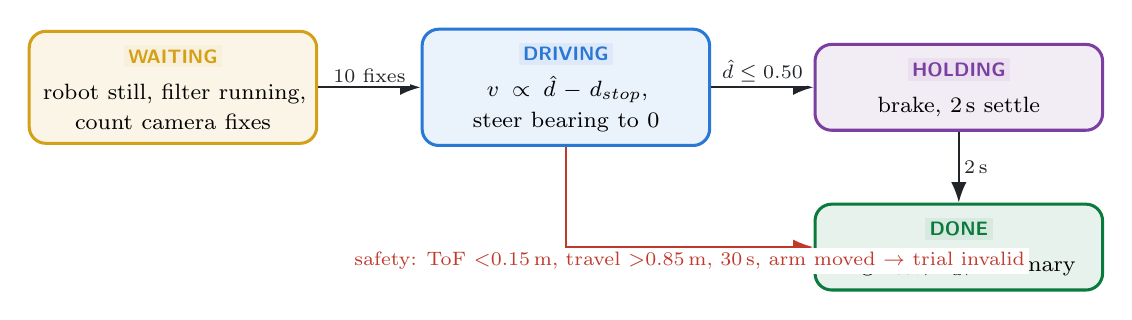
\begin{tikzpicture}[node distance=7mm and 13mm]
  \node[stnode=WAITING] (w) {\stbadge{WAITING}\\[2pt]\footnotesize robot still, filter running, count camera fixes};
  \node[stnode=DRIVING,right=of w] (d) {\stbadge{DRIVING}\\[2pt]\footnotesize $v\propto\dest-d_{stop}$, steer bearing to 0};
  \node[stnode=HOLDING,right=of d] (h) {\stbadge{HOLDING}\\[2pt]\footnotesize brake, 2\,s settle};
  \node[stnode=DONE,below=9mm of h] (n) {\stbadge{DONE}\\[2pt]\footnotesize log $d_{est}$, $\sigma_d$, summary};
  \draw[tr] (w) -- node[trl,above]{10 fixes} (d);
  \draw[tr] (d) -- node[trl,above]{$\dest\le0.50$} (h);
  \draw[tr] (h) -- node[trl,right]{2\,s} (n);
  \draw[tr,accred] (d.south) |- node[trl,pos=0.75,below]{safety: ToF $<$0.15\,m, travel $>$0.85\,m, 30\,s, arm moved $\rightarrow$ trial invalid} (n.west);
\end{tikzpicture}
\caption{Controller states (same colors in the video). No trial ended on a safety condition.}
\label{fig:fsm}
\end{figure}

%============================ 3. SETUP AND CALIBRATION ========================
\isec{\faTools}{Experimental Setup and Calibration}
\label{sec:setup}

\isub{\faCamera}{Camera pose}
The range calibration is only valid at one arm pose, so the arm is commanded to the saved pose
$(x,z)=(0.123,0.067)$\,m before every run and the controller refuses to drive if it is more than 6\,mm off.
Because the tag lies flat, its normal is the floor normal, and the detected tag pose gives the camera height and pitch
directly: \textbf{0.315\,m and 6.1$^\circ$ down} (Phase 2 had 5.3$^\circ$; the arm had been moved since). The pitch
$\beta=6.1^\circ$ is used in the level-frame rotation of Section~\ref{sec:method}.

\isub{\faRulerCombined}{Range calibration with the robot driving itself}
The camera's forward offset $f$ is mapped to the tape distance (chassis front to tag centre) by a straight line
$d = s f + o$. Instead of placing the robot by hand at five distances, a script
(\code{scripts/auto_calibrate_range.py}) drives the robot at 5\,cm/s, steering at the tag, and stops at
1.20, 1.00, 0.80, 0.60 and 0.50\,m; at each stop it averages 5\,s of camera readings. Only the first and last
positions need the tape; the stops in between are known from odometry and serve as a check.

\begin{table}[H]
\centering\small
\rowcolors{2}{kfupmlight}{white}
\begin{tabular}{@{}lrrrl@{}}
\rowcolor{kfupm}\hd{Stop} & \hd{Tape / odometry (m)} & \hd{Camera $f$ (m)} & \hd{Spread (mm)} & \hd{Use}\\
start & 1.200 (tape) & 1.3219 & 1.4 & fit anchor\\
1 & 0.9915 (odometry) & 1.1190 & 1.3 & check: fit residual $+3.2$\,mm\\
2 & 0.7787 (odometry) & 0.9120 & 0.6 & check: fit residual $+6.6$\,mm\\
last & 0.470 (tape) & 0.6003 & 0.2 & fit anchor\\
\end{tabular}
\caption{Range calibration, run 2 (\code{results/calibration/}). The fit through the two tape anchors gives
$s=1.0115$, $o=-0.1372$\,m for a 155\,mm tag size; with the measured 154\,mm the camera offsets scale by 154/155, so
$s=1.0181$ is used with the same $o$.}
\label{tab:calib}
\end{table}

\begin{itemize}
  \item \textbf{Run 1 was discarded.} Without steering the robot drifted on the rug and ended with the tag
        18$^\circ$ to the side; the camera gives the forward offset while the tape measures the diagonal, about
        2\,cm different at that angle. Steering was added to the script for run 2 (bearing stayed within
        0.2 to 0.4$^\circ$).
  \item \textbf{Run 2 had a Wi-Fi drop} of 3\,s during the leg to 0.60\,m; the robot kept its last speed and overshot
        to 0.47\,m, and \code{/odom} restarted from zero, so odometry after the drop was not used. This is why the
        fit uses the two tape anchors only.
  \item The two odometry check points sit 3 and 7\,mm above the fit, i.e.\ odometry over-reads the distance travelled
        by about 1.5\,\% on this rug (run 1 gave 2.1\,\%). This is the along-track drift the camera has to correct.
\end{itemize}

\isub{\faWrench}{Odometry: two driver problems found and fixed}
\label{sec:odomfix}
Three test drives (trial 0, kept in \code{results/test_runs/}) were made before the 10 trials.

\begin{table}[H]
\centering\small
\setlength{\tabcolsep}{4pt}
\rowcolors{2}{kfupmlight}{white}
\begin{tabularx}{\linewidth}{@{}l>{\raggedright\arraybackslash}Xrrrrr@{}}
\rowcolor{kfupm}\hd{Test} & \hd{Odometry source} & \hd{$d_{est}$} & \hd{camera} & \hd{wheels only} & \hd{tape} & \hd{$e$ (mm)}\\
1 & \code{/odom} twist ($v,\omega$ fields) & 0.514 & 0.535 & 0.158 & 0.540 & $-26$\\
2 & speed from \code{/odom} pose; one glitch at the stop & 0.614 & 0.500 & 0.507 & 0.520 & $+94$\\
3 & pose + plausibility guard (final setting) & 0.497 & 0.497 & 0.520 & 0.490 & $+7$\\
\end{tabularx}
\caption{Test drives that shaped the odometry input (distances in m).}
\label{tab:testruns}
\end{table}

\begin{itemize}
  \item \textbf{Twist is wrong and late.} At a true speed of 0.15\,m/s (from the camera) the twist field read
        0.18 to 0.21\,m/s, and at 0.03\,m/s it read 3 to 5 times too much, lagging by more than a second. Integrated, it
        put the robot 38\,cm past its real position. The \code{/odom} \emph{pose}, in contrast, agreed with the camera to
        1 to 2\,\% in both calibration runs, so the speed and turn rate are now differentiated from consecutive poses
        (\code{odom_source: pose}).
  \item \textbf{Pose glitches.} While standing still, one pose step gave $-0.72$\,m/s. The EKF moved 11\,cm, and the
        $\chi^2$ gate then rejected every correct camera reading (NIS 12.5) because they disagreed with the corrupted
        estimate. A plausibility guard now skips any odometry step faster than 0.40\,m/s or 1.5\,rad/s (more than
        twice what this controller ever commands); skipped steps are counted in \code{n_odom_glitches}.
\end{itemize}

\isub{\faClipboardList}{Protocol of a trial}
\begin{enumerate}
  \item Place the robot on the taped start marks (front edge on the 1.20\,m line, nose at the tag); arm at the saved pose.
  \item Run \code{ros2 launch rm_odom_ekf phase3.launch.py trial:=N}. Do not touch the robot until \stbadge{DONE}.
  \item Without moving the robot, tape from the middle of the chassis front to the tag centre; record with
        \code{scripts/add_measurement.py N} \textit{reading}.
  \item A trial is invalid if a safety stop ends it; it is then repeated with the same $N$.
\end{enumerate}
The configuration (\code{config/robot.yaml}) was not changed during the 10 trials.

%============================ 4. RESULTS ======================================
\isec{\faFlask}{Results of the 10 Trials}
\label{sec:results}

All 10 trials started from the same marks at 1.20\,m, ended with the normal stop
(\textit{EKF distance $\le$ 0.50\,m}, no safety stop) and lasted about 7.3\,s of driving. For each trial the robot
logged its final estimate $d_{est}$ with its uncertainty $\sigma_{EKF}$, and the distance was then measured with a tape
from the same reference point. The camera-only and wheels-only distances, logged in the same run, are listed for the
discussion.

\begin{table}[H]
\centering\small
\setlength{\tabcolsep}{5pt}
\rowcolors{2}{kfupmlight}{white}
\begin{tabular}{@{}crrrrr|rr|rr@{}}
\rowcolor{kfupm}\hd{Trial} & \hd{$d_{est}$ (m)} & \hd{$\sigma_{EKF}$ (cm)} & \hd{$d_{meas}$ (m)} & \hd{$e$ (cm)} & \hd{$|e|$ (cm)} &
  \hd{$e_{cam}$} & \hd{$e_{wheels}$} & \hd{glitches} & \hd{fixes (rej.)}\\
1  & 0.4968 & 0.88 & 0.492 & $+0.48$ & 0.48 & $+0.40$ & $+0.32$ & 0 & 196 (0)\\
2  & 0.4966 & 0.88 & 0.498 & $-0.14$ & 0.14 & $-0.16$ & $+0.76$ & 0 & 187 (0)\\
3  & 0.4948 & 0.96 & 0.495 & $-0.02$ & 0.02 & $-0.03$ & $-0.08$ & 0 & 184 (0)\\
4  & 0.4956 & 0.89 & 0.498 & $-0.24$ & 0.24 & $-0.25$ & $+0.09$ & 0 & 190 (0)\\
5  & 0.4802 & 0.88 & 0.485 & $-0.48$ & 0.48 & $-0.52$ & $-0.23$ & 0 & 203 (0)\\
6  & 0.4837 & 0.88 & 0.488 & $-0.43$ & 0.43 & $-0.54$ & $+5.81$ & 4 & 176 (0)\\
7  & 0.4774 & 0.88 & 0.480 & $-0.26$ & 0.26 & $-0.32$ & $-0.50$ & 0 & 190 (0)\\
8  & 0.4859 & 0.88 & 0.482 & $+0.39$ & 0.39 & $+0.24$ & $+4.82$ & 2 & 181 (0)\\
9  & 0.4953 & 0.95 & 0.495 & $+0.03$ & 0.03 & $-0.14$ & $+2.90$ & 2 & 205 (8)\\
10 & 0.4929 & 0.96 & 0.496 & $-0.31$ & 0.31 & $-0.30$ & $+4.25$ & 2 & 168 (0)\\
\midrule
\multicolumn{4}{r}{\textbf{MAE}} & \multicolumn{2}{r|}{\textbf{0.28\,cm}} & 0.29 & 1.98 & & \\
\multicolumn{4}{r}{\textbf{Range of errors}} & \multicolumn{2}{r|}{\textbf{0.96\,cm}} & 0.95 & 6.31 & & \\
\end{tabular}
\caption{Final distance in every trial. $e = d_{est}-d_{meas}$ is the graded error. $e_{cam}$: last camera reading
alone; $e_{wheels}$: wheel odometry alone, never corrected (both in cm, same runs). ``Glitches'': odometry steps
skipped by the guard; ``fixes'': camera corrections used (rejected by the gate). Generated from
\code{results/summary_table.csv}.}
\label{tab:trials}
\end{table}

\begin{center}
\begin{minipage}{\linewidth}
\stat[kfupm]{\faBullseye}{0.28\,cm}{mean absolute error}\hfill
\stat[accblue]{\faArrowsAltH}{0.96\,cm}{range, $-0.48$ to $+0.48$}\hfill
\stat[accpurple]{\faBalanceScale}{$-0.10$\,cm}{bias $\bar e$ (p = 0.36)}\hfill
\stat[accorange]{\faChartArea}{0.32\,cm}{std.\ deviation $\sigma$}
\end{minipage}
\end{center}

%-----------------------------------------------------------------------------
\isub{\faBullseye}{The scatter plot: estimate against tape}
\begin{figure}[H]
\centering
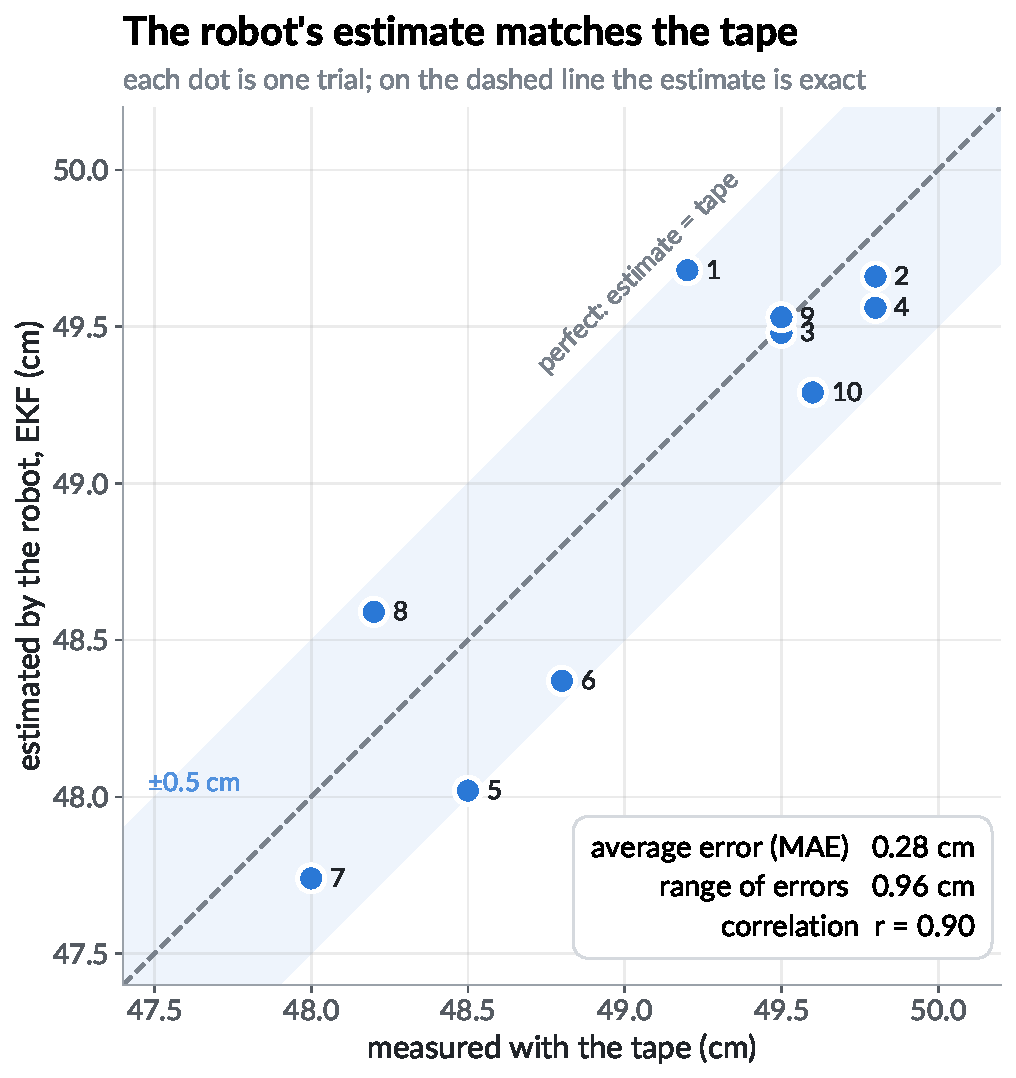
\includegraphics[width=0.66\linewidth]{figures/simple_1_scatter.pdf}
\caption{Estimated versus measured final distance, one dot per trial.
\textbf{How to read it:} on the dashed line the estimate equals the tape; the shaded band is $\pm$0.5\,cm.
All ten dots are inside the band, and they follow the line even though the robot stopped at different places
(47.8 to 49.8\,cm) because it coasted after braking.}
\label{fig:scatter}
\end{figure}

\begin{figure}[H]
\centering
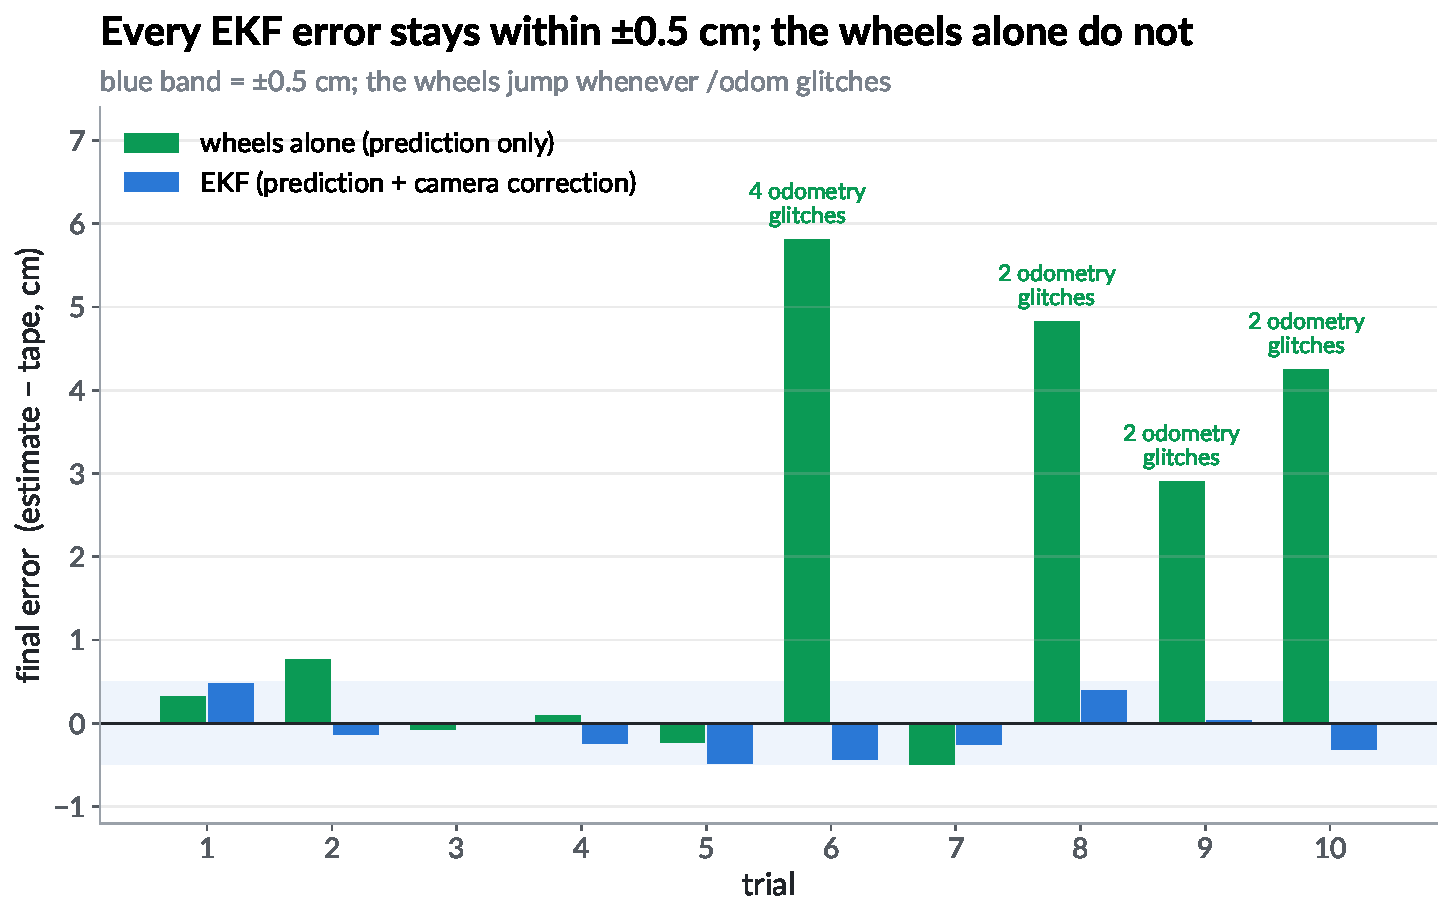
\includegraphics[width=0.92\linewidth]{figures/simple_2_per_trial.pdf}
\caption{Final error of every trial for the EKF (blue) and for the wheels alone (green).
\textbf{How to read it:} the closer a bar is to zero, the better. The EKF bars all stay in the $\pm$0.5\,cm band.
The wheels alone are as good in trials 1 to 5 and 7, but jump to 2.9 to 5.8\,cm in the four trials in which \code{/odom}
glitched: odometry has no way to notice its own error, the camera correction does.}
\label{fig:errors}
\end{figure}

%-----------------------------------------------------------------------------
\isub{\faCalculator}{Statistical analysis}
\label{sec:stats}
With $N=10$ trials and $e_i = d_{est,i}-d_{meas,i}$:
\begin{equation}
\text{MAE}=\frac1N\sum_{i=1}^{N}|e_i|,\quad \text{range}=\max_i e_i-\min_i e_i,\quad
\bar e=\frac1N\sum e_i,\quad s=\sqrt{\tfrac{1}{N-1}\textstyle\sum (e_i-\bar e)^2},\quad
\text{RMSE}=\sqrt{\tfrac1N\textstyle\sum e_i^2}.
\end{equation}

\begin{table}[H]
\centering\small
\setlength{\tabcolsep}{6pt}
\rowcolors{2}{kfupmlight}{white}
\begin{tabular}{@{}lrrrrrr@{}}
\rowcolor{kfupm}\hd{Method} & \hd{MAE} & \hd{bias $\bar e$} & \hd{std.\ dev.\ $s$} & \hd{RMSE} & \hd{min / max} & \hd{range}\\
\textbf{EKF (predict + correct)} & \textbf{0.28} & $-0.10$ & 0.32 & 0.32 & $-0.48$ / $+0.48$ & \textbf{0.96}\\
Camera alone & 0.29 & $-0.16$ & 0.30 & 0.33 & $-0.54$ / $+0.40$ & 0.95\\
Wheels alone & 1.98 & $+1.81$ & 2.39 & 2.91 & $-0.50$ / $+5.81$ & 6.31\\
\end{tabular}
\caption{Descriptive statistics of the final error, in cm.}
\label{tab:descr}
\end{table}

\begin{figure}[H]
\centering
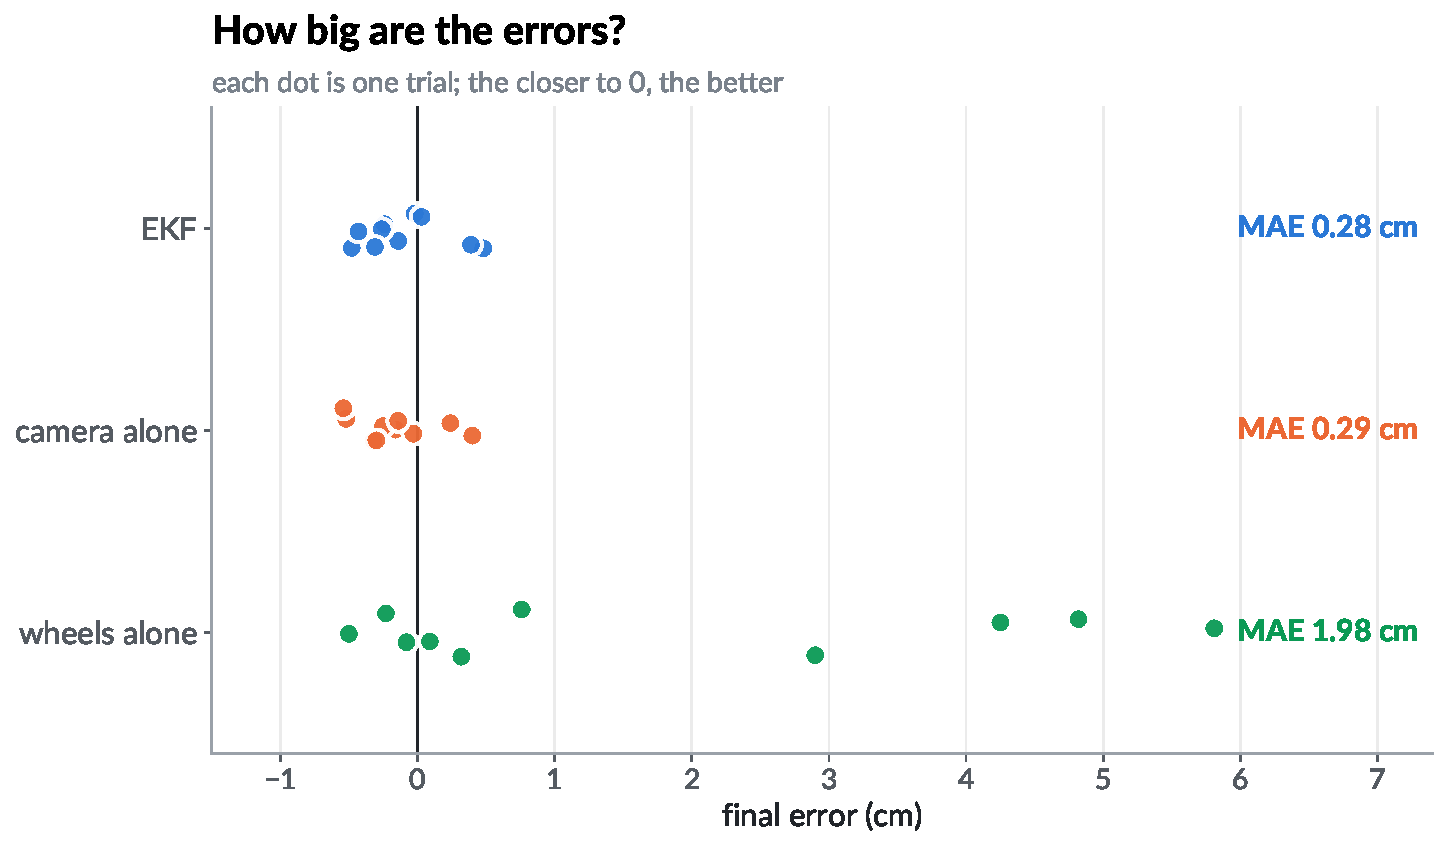
\includegraphics[width=0.84\linewidth]{figures/simple_3_spread.pdf}
\caption{All 30 errors on one axis. \textbf{How to read it:} each dot is a trial; a tight cluster around zero means an
accurate and repeatable method. The EKF and the camera form a tight cluster within half a centimetre; the wheels alone
spread over six centimetres.}
\label{fig:spread}
\end{figure}

\lead{Is there a systematic error (bias)?} A one-sample $t$-test of $H_0: \bar e = 0$ gives $t=-0.96$, $p=0.36$ for
the EKF; the 95\,\% confidence interval of the mean error is $[-0.33,\ +0.13]$\,cm and contains zero. \emph{The EKF has no
detectable bias.} The wheels alone have a significant bias of $+1.81$\,cm ($t=2.40$, $p=0.04$, interval
$[+0.10,\ +3.53]$\,cm): when odometry steps are lost, the wheels under-count the travel and think the robot is farther from
the tag than it is.

\lead{Does the estimate follow reality?} A least-squares fit of $d_{est}$ on $d_{meas}$ gives a slope of
$0.99 \pm 0.17$ (standard error), an intercept of 0.23\,cm and $R^2=0.81$ ($p=0.0004$); the Pearson correlation is
$r=0.90$ and the covariance $\operatorname{cov}(d_{est},d_{meas})=0.445$\,cm$^2$. A slope of one means that when the robot
really stops 1\,cm earlier, the estimate also says 1\,cm earlier.

\lead{Is the EKF better than the wheels alone?} In spread, clearly: the variance ratio is
$F = s^2_{wheels}/s^2_{EKF} = 54.6$ ($p<0.001$; Levene's test $p=0.013$). In absolute error the Wilcoxon signed-rank test
gives $p=0.084$: with ten trials and odometry already good in six of them, the difference in \emph{typical} error is not
significant at 5\,\%, while the difference in \emph{reliability} (worst case 0.48 against 5.81\,cm) is. Against the camera
alone the EKF is not different ($p=0.38$), as expected when the camera sees the tag until the stop
(Section~\ref{sec:role}). The EKF errors are compatible with a normal distribution (Shapiro--Wilk $p=0.28$).

\begin{figure}[H]
\centering
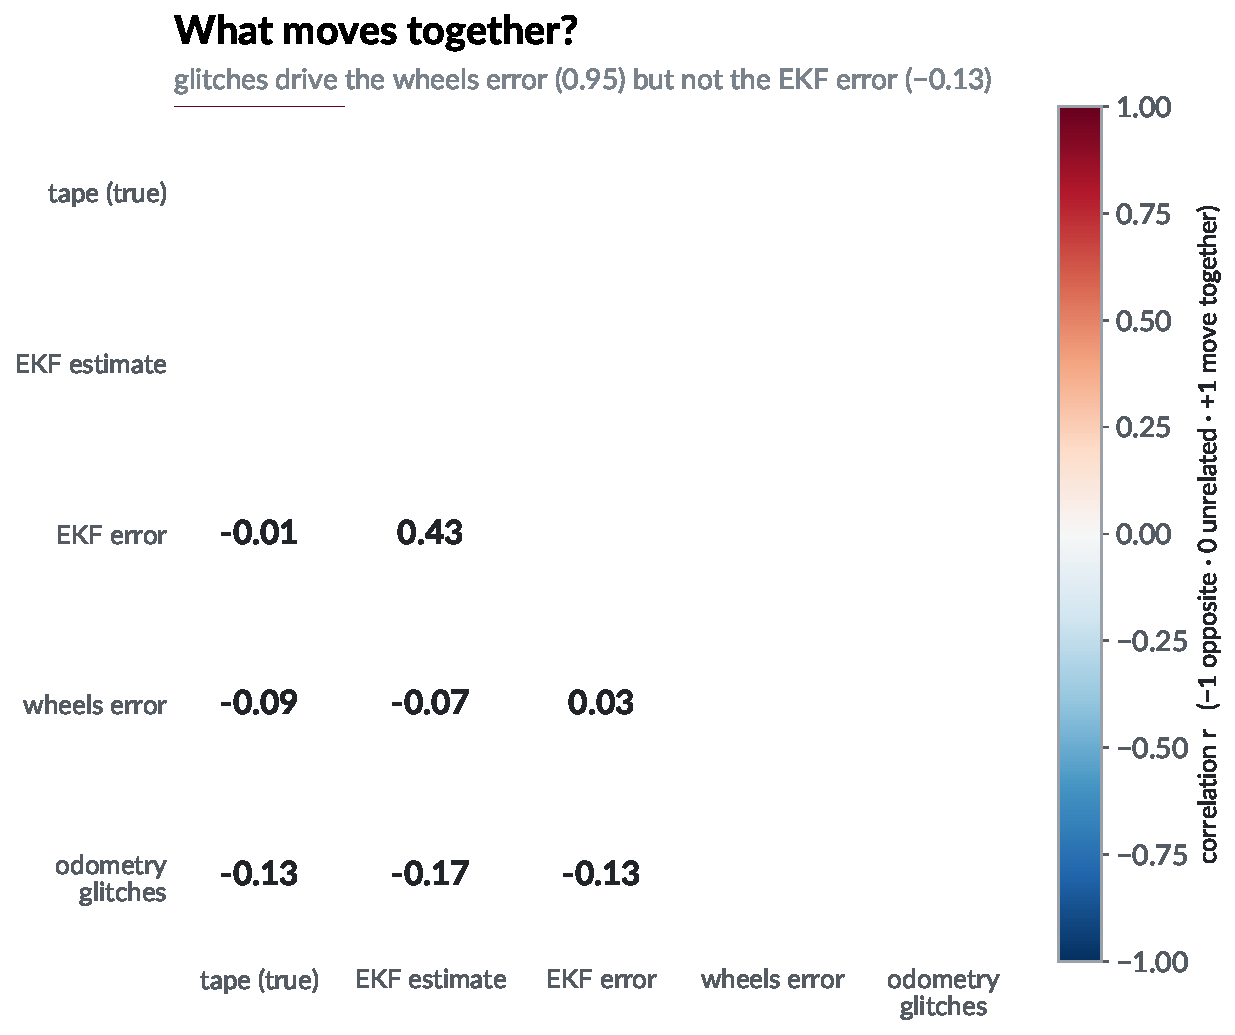
\includegraphics[width=0.70\linewidth]{figures/simple_4_correlation.pdf}
\caption{Correlation matrix of five per-trial quantities. \textbf{How to read it:} $+1$ means two quantities rise
together, 0 means unrelated. Three cells tell the story: estimate and tape move together (0.90); the wheels error is
driven by the odometry glitches (0.95); the EKF error is not ($-0.13$), because the camera correction removes what the
glitches add.}
\label{fig:corr}
\end{figure}

\begin{figure}[H]
\centering
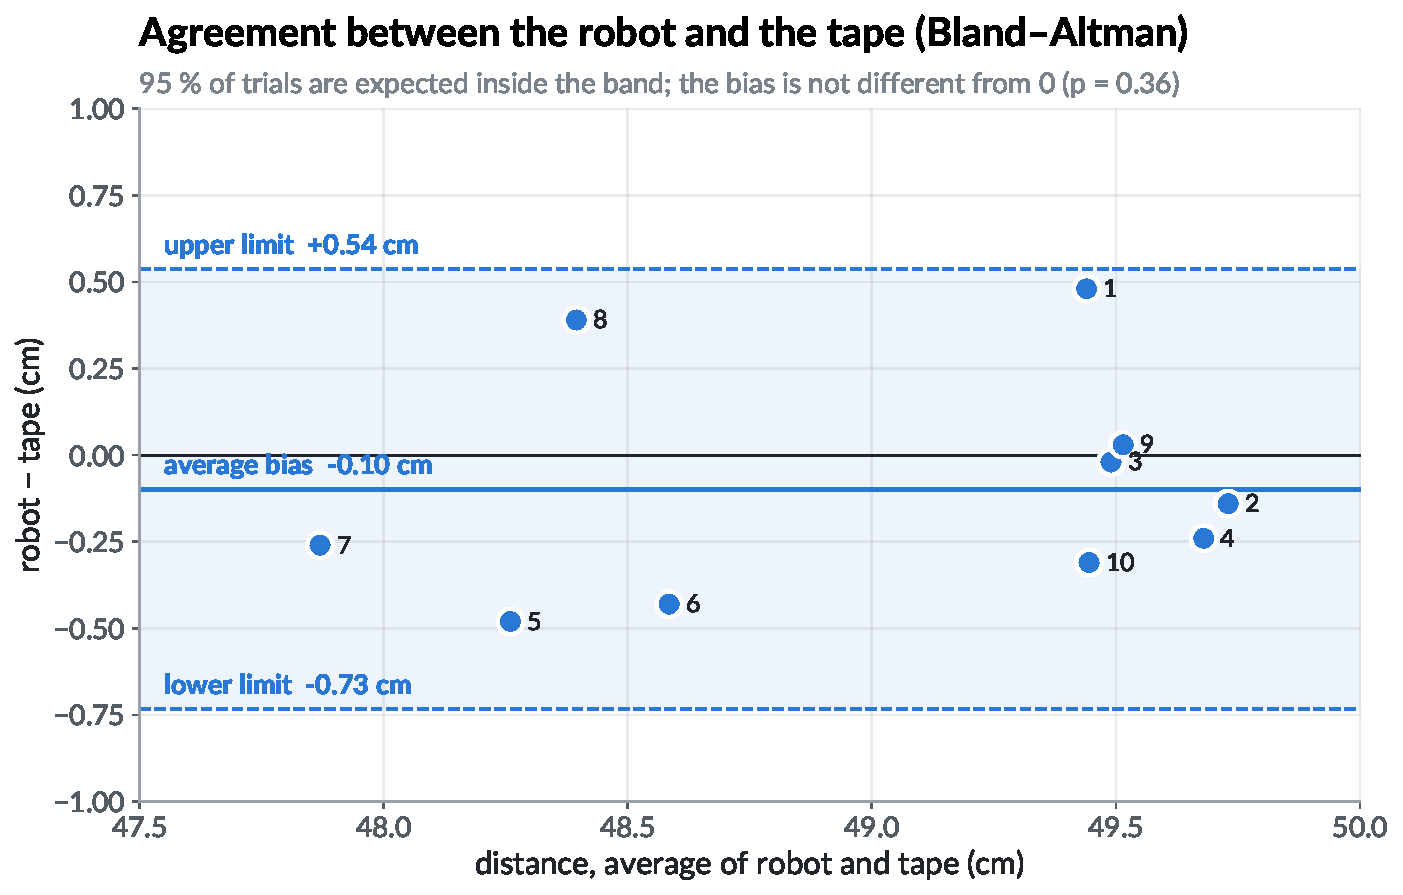
\includegraphics[width=0.84\linewidth]{figures/simple_5_agreement.pdf}
\caption{Bland--Altman plot, the standard way to compare two methods that measure the same quantity.
\textbf{How to read it:} each dot is a trial, the vertical axis is how far the robot is from the tape. The solid line is
the average bias ($-0.10$\,cm) and the dashed lines are the 95\,\% limits of agreement, $-0.73$ to $+0.54$\,cm: a new
trial is expected to agree with the tape within this band. The differences do not grow with the distance, so there is no
scale error.}
\label{fig:ba}
\end{figure}

\begin{notebox}
\small\lead{Why no confusion matrix?} A confusion matrix counts right and wrong \emph{class} decisions. This experiment
measures a continuous distance, so agreement is assessed with the scatter plot and regression, the Bland--Altman
limits of agreement and the correlation matrix above.
\end{notebox}

%-----------------------------------------------------------------------------
\isub{\faChartLine}{During the drive}
\begin{figure}[H]
\centering
\begin{subfigure}[t]{0.49\linewidth}\centering
  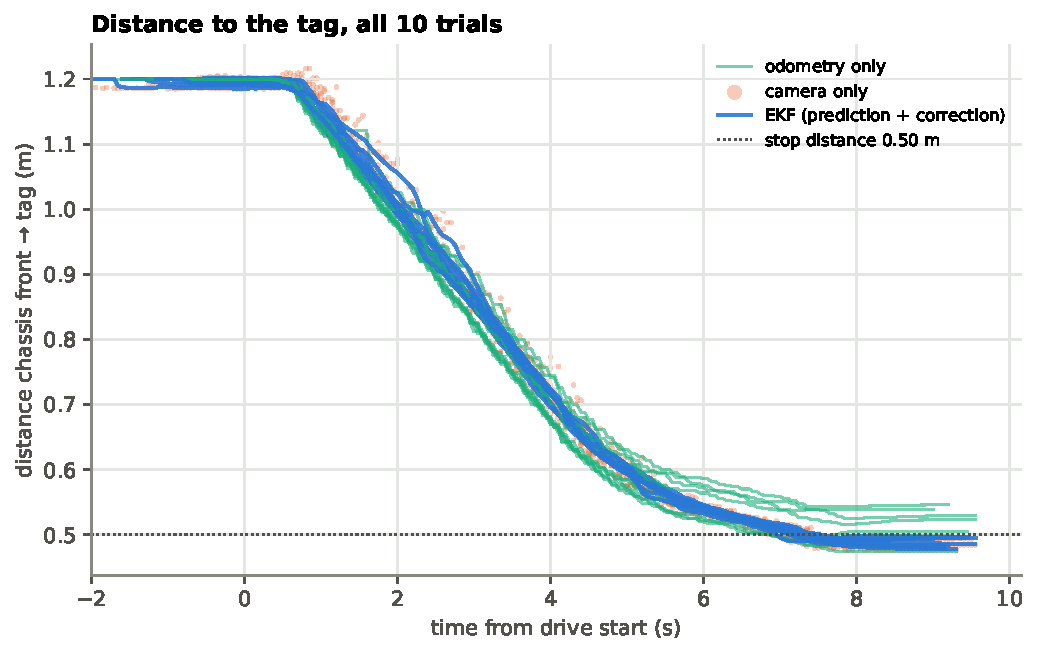
\includegraphics[width=\linewidth]{figures/fig3_distance_vs_time.pdf}
  \caption{Distance to the tag during every trial.}
  \label{fig:dist}
\end{subfigure}\hfill
\begin{subfigure}[t]{0.49\linewidth}\centering
  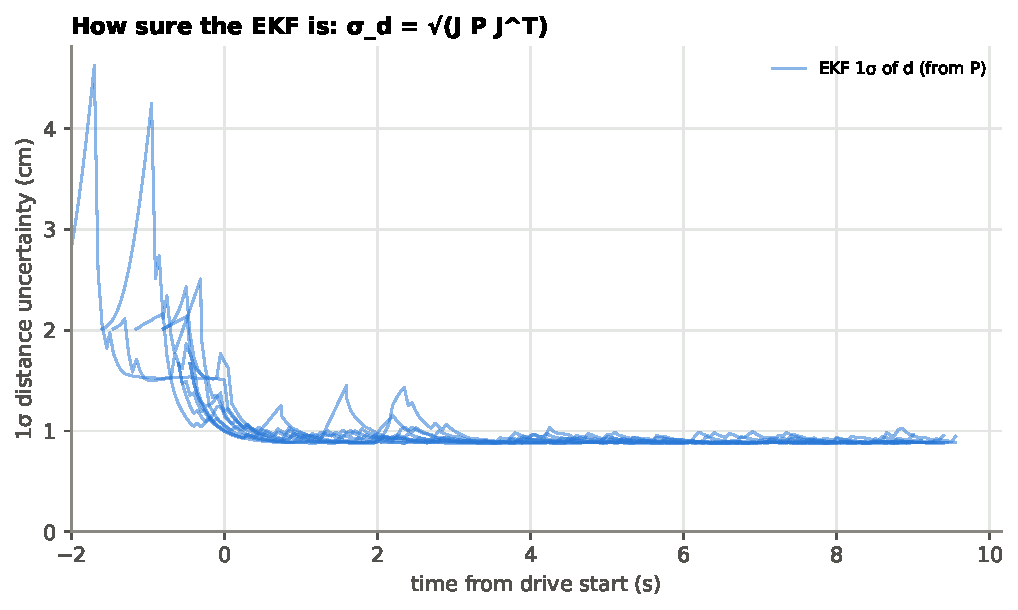
\includegraphics[width=\linewidth]{figures/fig4_ekf_uncertainty.pdf}
  \caption{EKF uncertainty $\sigma_d$ during every trial.}
  \label{fig:sigma}
\end{subfigure}
\caption{Time histories. The uncertainty starts at the placement accuracy, drops as soon as the camera fixes arrive,
and stays below 1\,cm while driving because a camera correction arrives every 70\,ms on average.}
\label{fig:stats}
\end{figure}

\begin{figure}[H]
\centering
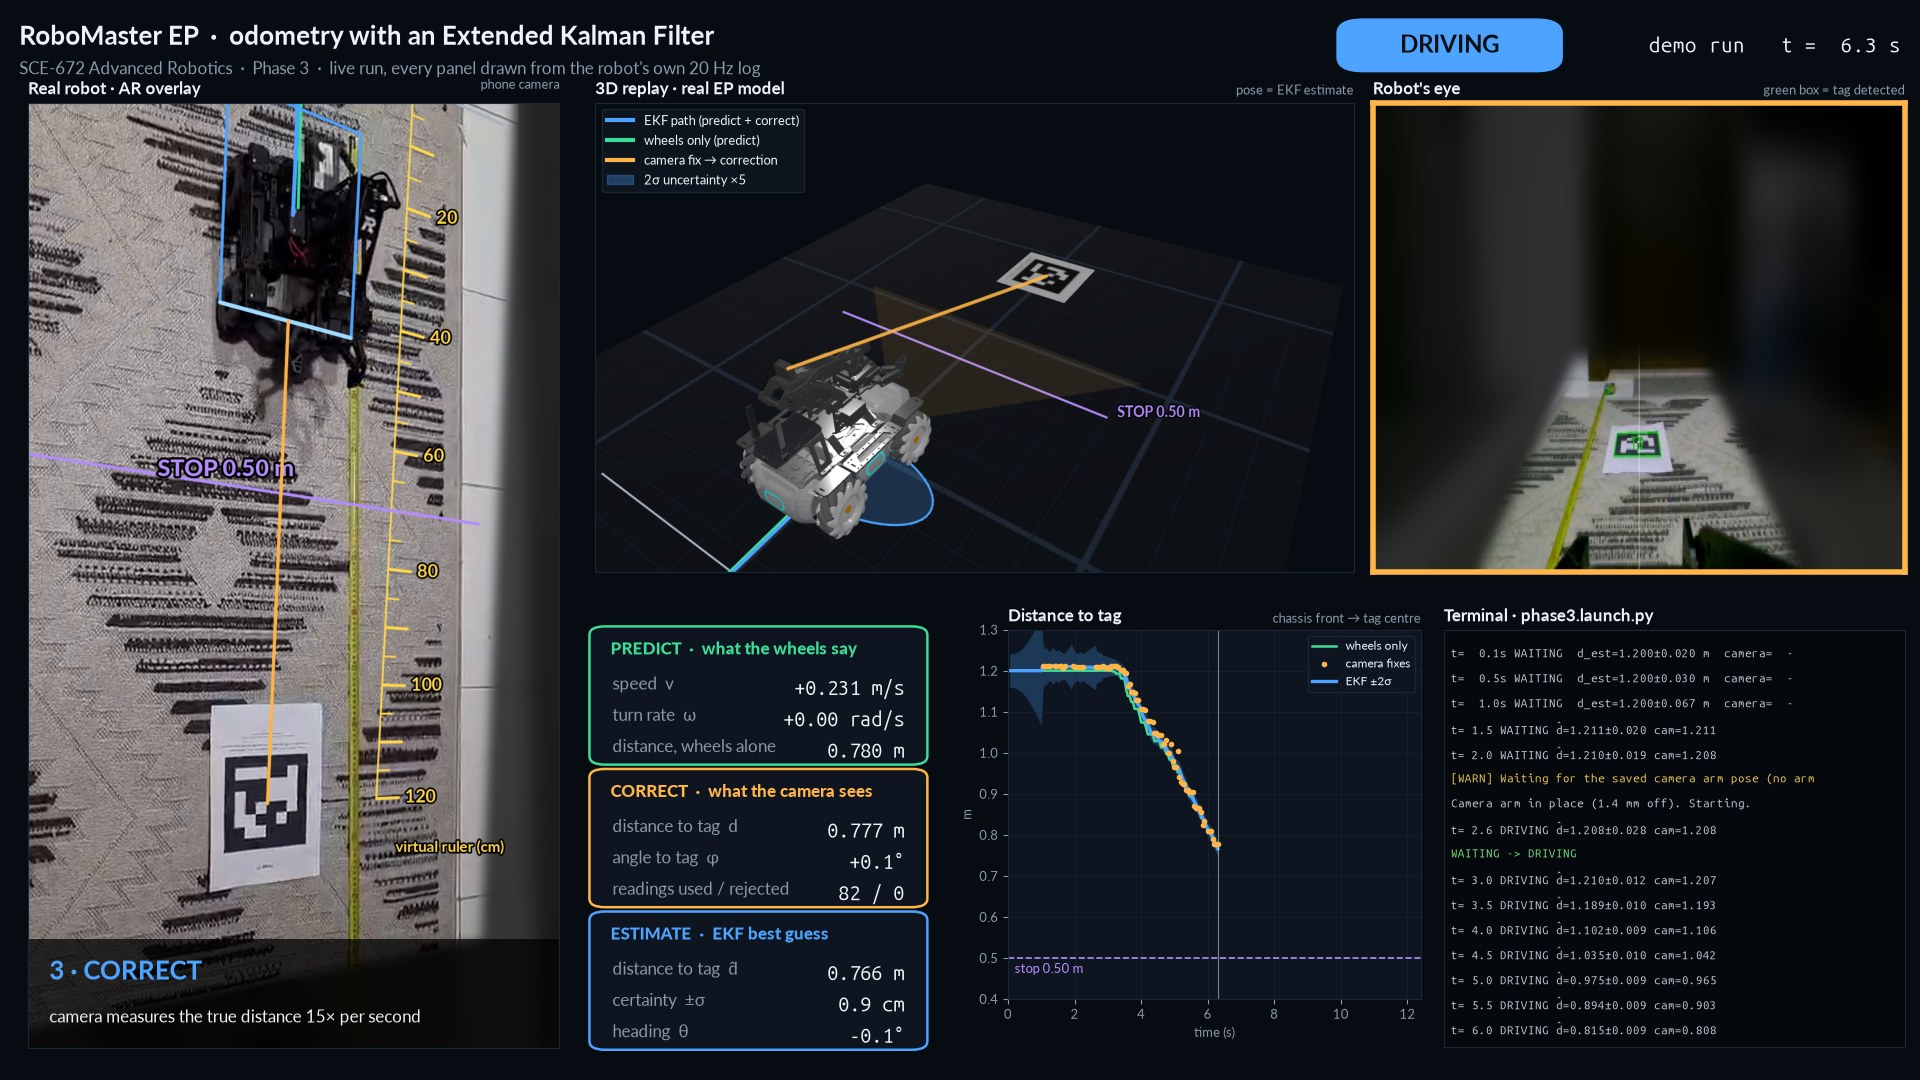
\includegraphics[width=\linewidth]{figures/still_driving.jpg}
\caption{Frame of the demo video (\link{\videolink}{link}). Left: phone video with an augmented-reality overlay drawn
on the floor from the tag's own pose (blue outline: the EKF estimate of the robot footprint; yellow: virtual ruler
next to the real tape; orange: the current camera correction). Right: 3D replay with DJI's EP model, the robot's camera,
the three groups of numbers, the distance history and the terminal.}
\label{fig:video}
\end{figure}

%============================ 5. DISCUSSION ===================================
\isec{\faComments}{Discussion}
\label{sec:discussion}

\isub{\faEquals}{Consistency of the trials}
The ten errors lie between $-0.48$ and $+0.48$\,cm, with a standard deviation of 0.32\,cm and a mean of
$-0.10$\,cm. The mean is smaller than its own standard error ($0.32/\sqrt{10}=0.10$\,cm), so there is no evidence of a
systematic offset: the remaining error is scatter, not bias.

Where the robot \emph{stopped} varied much more than how well it \emph{knew} where it stopped. The tape readings range
from 0.480 to 0.498\,m: in trials 5 to 8 the robot coasted 1.4 to 2.2\,cm past the brake point after the speed command went
to zero. The estimate followed this coasting in every case (correlation 0.90 between $d_{est}$ and $d_{meas}$), so the
stopping error belongs to the controller and the chassis, not to the estimator. Stopping more precisely would need a
lower final speed or braking earlier; it would not change the estimation error that this project measures.

\isub{\faSearch}{Sources of error}
\begin{table}[H]
\centering\small
\setlength{\tabcolsep}{4pt}
\rowcolors{2}{kfupmlight}{white}
\begin{tabularx}{\linewidth}{@{}>{\raggedright\arraybackslash}p{3.2cm}>{\raggedright\arraybackslash}X>{\raggedright\arraybackslash}p{3.6cm}@{}}
\rowcolor{kfupm}\hd{Source} & \hd{Evidence in this project} & \hd{Effect and handling}\\
Wheel slip on the rug & odometry over-reads the travel by 1.5 to 2.1\,\% (both calibration runs) & along-track drift; corrected by the camera range\\
Odometry glitches & 10 impossible pose steps in trials 6, 8, 9, 10; wheels-only error 2.9 to 5.8\,cm there & guard skips them; camera removes the lost travel\\
\code{/odom} twist field & 20 to 40\,\% too high and over 1\,s late; 38\,cm error in test 1 & not used; speed from the pose\\
Camera range calibration & fit through two tape anchors; check points within 3 and 7\,mm & residual bias, shared by EKF and camera (both $\approx$0.3\,cm)\\
Camera detection limits & tag 10\,px tall at 1.5\,m (unreliable), lost below 0.47\,m & start 1.20\,m, stop 0.50\,m\\
Camera outliers & 8 readings with NIS $>$ 9.21 in trial 9 & $\chi^2$ gate\\
Wi-Fi drops & 3\,s drop in calibration: robot kept moving 14\,cm, \code{/odom} reset & none in the 10 trials; such a trial would be repeated\\
Tape reading & read to about $\pm$2 to 3\,mm from the chassis front & of the same size as $\sigma=3.2$\,mm\\
Controller coasting & 1.4 to 2.2\,cm past the brake point in trials 5 to 8 & stopping error, tracked by the estimate\\
\end{tabularx}
\caption{Error sources, each with the evidence for it.}
\label{tab:sources}
\end{table}

The final error of 0.28\,cm is about the size of the tape reading uncertainty, so the result should be read as
\emph{the estimate agrees with the tape to within the resolution of the tape}, not as millimetre accuracy.

\isub{\faBalanceScaleLeft}{Role of prediction and correction}
\label{sec:role}
To separate what each part contributes, the logged inputs of the 10 trials were fed again through the same
\code{RobotEKF} code with one ingredient removed (\code{scripts/replay_ekf.py}). Replaying the unchanged filter
reproduces the logged estimate to within 0.04\,mm, so the differences below are caused only by the removed ingredient.

\begin{table}[H]
\centering\small
\rowcolors{2}{kfupmlight}{white}
\begin{tabular}{@{}lrrrr@{}}
\rowcolor{kfupm}\hd{Filter variant (same 10 trials)} & \hd{MAE (cm)} & \hd{bias (cm)} & \hd{$\sigma$ (cm)} & \hd{worst $|e|$ (cm)}\\
\textbf{As run: prediction + odometry + camera range and bearing} & \textbf{0.28} & $-0.10$ & 0.32 & 0.48\\
Camera noise $R_{tag}\times3$ & 0.25 & $+0.16$ & 0.31 & 0.68\\
Camera noise $R_{tag}/3$ & 0.30 & $-0.13$ & 0.34 & 0.54\\
Camera only, last reading, no filter & 0.30 & $-0.15$ & 0.33 & 0.55\\
Camera lost below 0.90\,m (prediction carries the last 40\,cm) & 1.86 & $+1.17$ & 1.64 & 2.72\\
Camera bearing only, no range & 1.98 & $-0.95$ & 2.63 & 4.92\\
No camera while driving (prediction + odometry) & 2.53 & $-1.52$ & 3.12 & 6.20\\
\end{tabular}
\caption{Offline replay: final-distance error with parts of the filter removed (\code{results/replay/}).}
\label{tab:replay}
\end{table}

\begin{figure}[H]
\centering
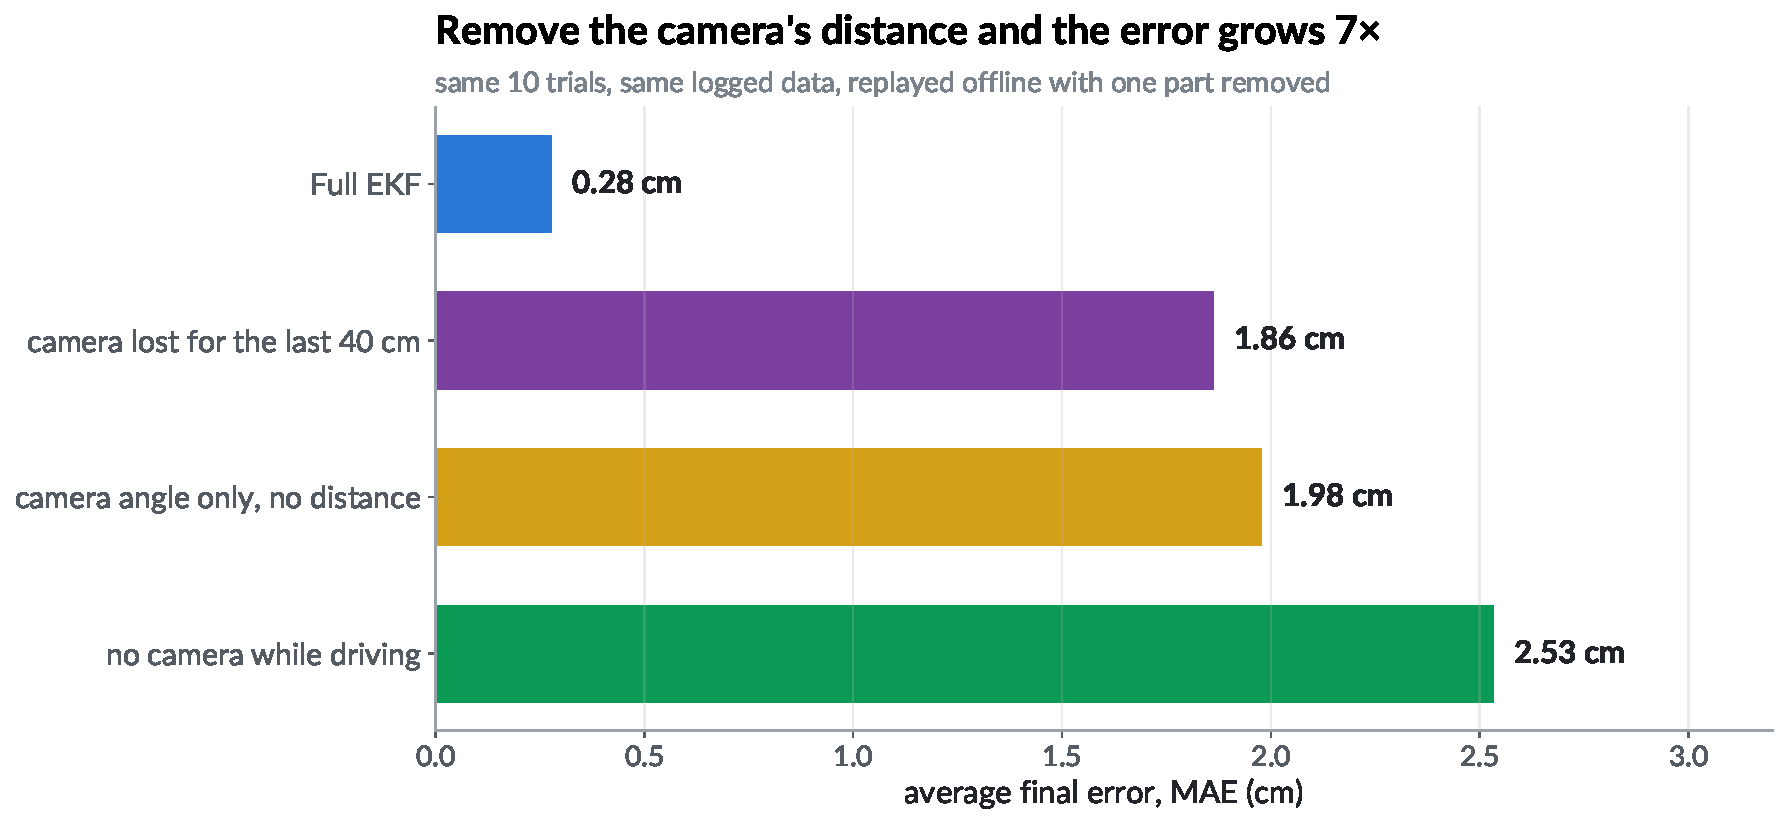
\includegraphics[width=0.86\linewidth]{figures/simple_6_contrib.pdf}\\[6pt]
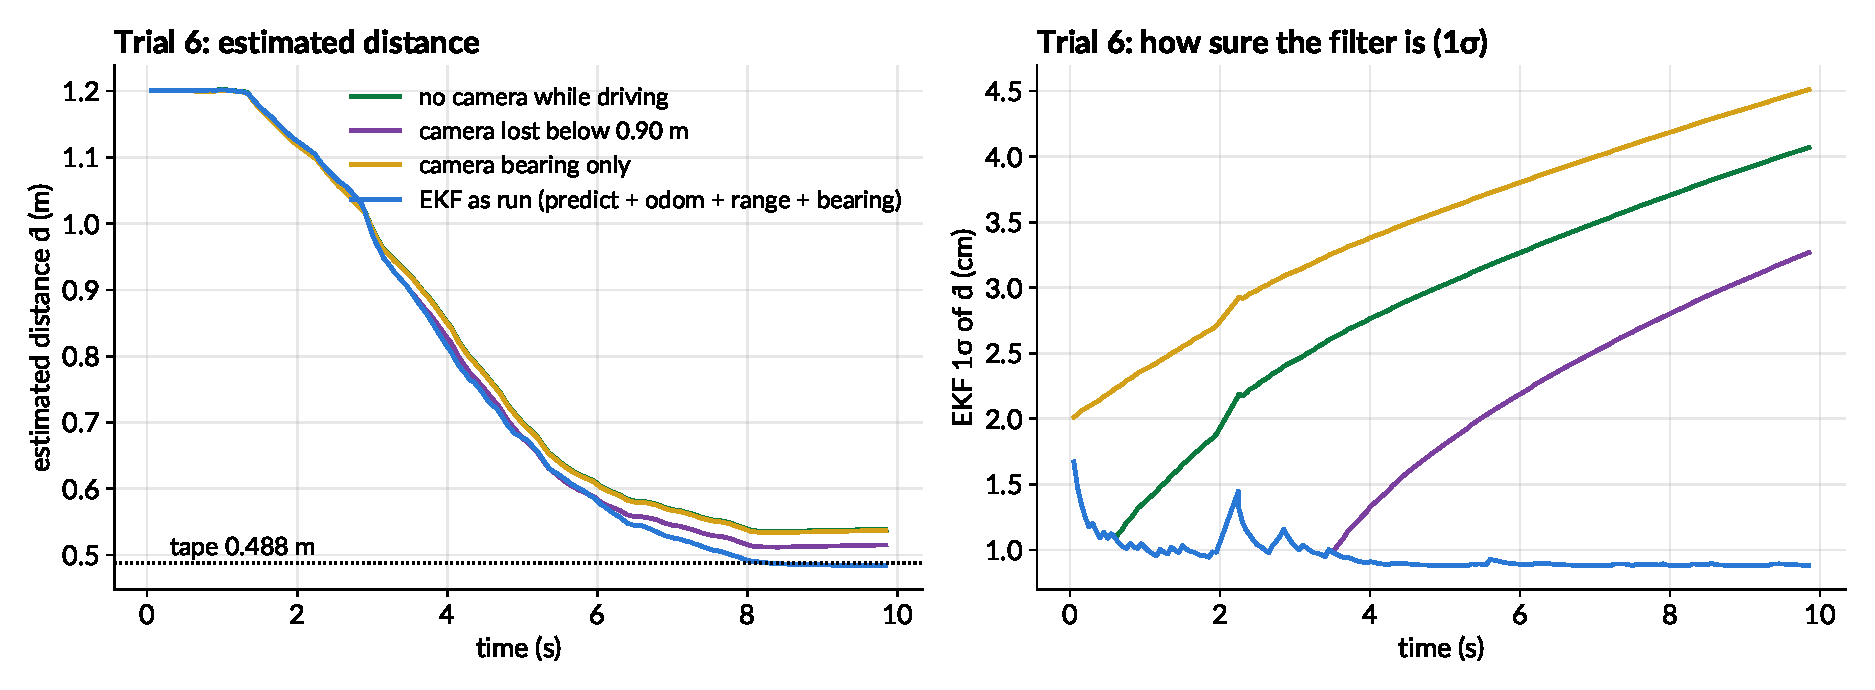
\includegraphics[width=0.92\linewidth]{figures/fig_replay_trial6.pdf}
\caption{Top: average final error when one part of the filter is removed. \textbf{How to read it:} shorter is better;
each bar is the same 10 trials replayed. Bottom: trial 6 replayed. Without the camera (green) the estimate drifts away
from the tape and its uncertainty $\sigma_d$ keeps growing; with the camera (blue) every correction pulls it back and
keeps $\sigma_d$ below 1\,cm.}
\label{fig:replay6}
\end{figure}

\lead{Prediction.} The motion model with odometry gives a smooth estimate at 20\,Hz, between camera fixes and through
any gap. On its own it is not enough: with no camera while driving the final error grows to 2.5\,cm on average and
6.2\,cm in the worst trial, and $\sigma_d$ grows with the distance driven (Figure~\ref{fig:replay6}). Two kinds of
odometry error cause this: slow drift from slip (about 1.5 to 2\,\% of the distance) and sudden glitches. Prediction is
also what makes the correction safe: the gate can reject a bad camera reading only because the prediction says where
the tag should be.

\lead{Correction.} The camera range bounds the along-track error at every fix, so the final error does not depend on
how far the robot drove or on how many odometry steps were lost. Trial 6 shows this directly: the wheels alone end
5.8\,cm off, the EKF 0.4\,cm.

\lead{Why range is required (Lecture 12A, slide 26).} Driving straight at the tag, $\Delta y\approx0$, so the bearing row
of $H_{tag}$ is $[\,0,\ -1/d,\ -1,\ 0,\ 0\,]$: its $p_x$ entry is zero, and bearing carries no information about the
distance along the line, which is exactly where odometry drifts. Only the range row $[-1,0,0,0,0]$ observes it.
The replay confirms it: bearing only gives 1.98\,cm, almost as bad as no camera at all (2.53\,cm), while range and bearing
give 0.28\,cm.

\lead{EKF versus the camera alone.} At the final position, the EKF (0.28\,cm) and the last camera reading (0.30\,cm) are
nearly equal. This is expected here, because the camera sees the tag until the stop, and the estimate at rest is
dominated by many camera fixes. The value of the filter is in what the camera alone cannot do: give an estimate at
every control tick with a known uncertainty, reject outliers, survive odometry glitches, and keep a usable estimate when
the camera is lost (1.86\,cm after 40\,cm without the camera, against no estimate at all).

\isub{\faHeartbeat}{Is the filter's uncertainty honest?}
\label{sec:consistency}
The filter reports $\sigma_d=0.90$\,cm at the stop, while the real spread is 0.32\,cm (ratio 0.36), and all 10 errors are
inside $\pm2\sigma_d$. The filter is therefore cautious rather than overconfident, which is the safe side: an overconfident
filter would start rejecting good camera readings at the gate. The replay with $R_{tag}\times3$ and $R_{tag}/3$ changes
the MAE by only 0.05\,cm, so the result does not hinge on the exact noise values. A tighter $R_{tag}$ (about 1\,cm
instead of 3\,cm) would bring $\sigma_d$ closer to the observed spread.

\isub{\faExclamationTriangle}{Limitations and transparency}
\begin{warnbox}
\small
\begin{itemize}
  \item \textbf{Two trials were repeated.} Trials 5 and 9 were run a second time after the first tape reading disagreed
        with the estimate by 12 and 10\,mm. Both first attempts are kept in \code{results/test_runs/} with their readings.
        If the first attempts are used instead, the MAE is 0.45\,cm, $\sigma$ = 0.59\,cm and the range $-1.19$ to
        $+0.99$\,cm; the conclusions do not change.
  \item \textbf{Same tape, same reference point.} The camera was calibrated against the same tape and reference point
        that later measured the trials, so the statistics measure repeatability and calibration residual rather than
        accuracy against an independent instrument.
  \item \textbf{Single geometry.} One start distance, one floor and one tag; the camera-limited stop at 0.50\,m was chosen
        for this tag size.
\end{itemize}
\end{warnbox}

%============================ 6. CONCLUSIONS ==================================
\isec{\faFlagCheckered}{Conclusions}
\label{sec:conclusions}

\begin{keybox}{\faCheckCircle\ \ Findings}
\begin{itemize}
  \item The RoboMaster detected the floor tag, drove straight to it from 1.20\,m and stopped before it in 10 of 10
        trials, using a 5-state EKF predicted with a unicycle model and corrected by wheel odometry and by the tag's
        range and bearing.
  \item The final distance estimate agreed with the tape to \textbf{0.28\,cm MAE}, with a \textbf{range of 0.96\,cm}
        ($-0.48$ to $+0.48$\,cm), no measurable bias and $\sigma=0.32$\,cm, about the resolution of the tape itself.
  \item Wheel odometry alone ended 1.98\,cm off on average and up to 5.8\,cm, because of slip on the rug and pose
        glitches in the driver.
  \item The camera \emph{range} is what fixes the along-track error. With bearing only the error rises to 1.98\,cm,
        close to having no camera at all (2.53\,cm), which matches the observability argument of Lecture 12A.
  \item Prediction provides the continuous, uncertainty-aware estimate that the controller and the outlier gate rely
        on, and it carries the estimate through camera gaps; correction keeps it from drifting.
\end{itemize}
\end{keybox}

\lead{What made the difference in practice.} Three problems were found and fixed before the trials, each visible in
the logs: the \code{/odom} twist field is late and too large (speed is now taken from the pose), the pose has rare
impossible jumps (now skipped by a plausibility guard), and a 154\,mm flat tag is unreliable beyond 1.2\,m with this
camera (start moved to 1.20\,m, stop to 0.50\,m).

\lead{Next steps.} Tighten $R_{tag}$ to about 1\,cm so that the reported $\sigma_d$ matches the observed spread; add a
final slow approach to remove the 1.5 to 2\,cm coasting at the stop; check absolute accuracy with an instrument independent
of the calibration (for example a second camera or a laser distance meter).

%============================ APPENDIX ========================================
\appendix
\isec{\faGithub}{Code, Data and Reproduction}
\label{sec:repro}

\begin{table}[H]
\centering\small
\rowcolors{2}{kfupmlight}{white}
\begin{tabularx}{\linewidth}{@{}l>{\raggedright\arraybackslash}X@{}}
\rowcolor{kfupm}\hd{Path} & \hd{Content}\\
\code{src/rm_odom_ekf/rm_odom_ekf/ekf.py} & the EKF: $f$, $F$, $G$, $H_{odom}$, $h$, $H_{tag}$, gate, update, wrap\\
\code{.../phase3_node.py} & ROS node: predict, odometry update, camera update, control, logging\\
\code{.../controller.py}, \code{tag_detector.py} & controller states; AprilTag range and bearing\\
\code{src/rm_odom_ekf/config/robot.yaml} & every parameter used in the trials\\
\code{src/rm_odom_ekf/test/} & 23 unit tests, including central-difference checks of $F$, $G$, $H_{tag}$\\
\code{results/trials/} & 10 trials: \code{steps.csv} (20\,Hz) and \code{summary.json}\\
\code{results/test_runs/}, \code{results/calibration/} & test drives, repeated first attempts, calibration data\\
\code{scripts/analyze_trials.py} & Table~\ref{tab:trials}, statistics, Figures~\ref{fig:scatter}--\ref{fig:stats}\\
\code{scripts/replay_ekf.py} & sensor-removal study, Table~\ref{tab:replay}\\
\code{theory/FORMULA_MAP.md} & every equation of this report and the code line that implements it\\
\code{video_tools/} & demo video: AR overlay, 3D replay, dashboard\\
\end{tabularx}
\caption{Repository: \link{\repoURL}{\repoURL}. Demo video: \link{\videolink}{\videolink}.}
\end{table}

\begin{lstlisting}[style=sh]
# unit tests (no robot needed)
cd src/rm_odom_ekf && python3 -m pytest -q test          # 23 passed
# one trial on the robot (driver running)
ros2 launch rm_odom_ekf phase3.launch.py trial:=N
python3 scripts/add_measurement.py N 0.492              # tape reading in metres
# statistics, figures and the replay study
python3 scripts/analyze_trials.py
python3 scripts/replay_ekf.py
\end{lstlisting}


\end{document}
